\documentclass[12pt, a4paper]{article}
\usepackage[francais]{babel}
\usepackage{caption}
\usepackage{graphicx}
\usepackage[T1]{fontenc}
\usepackage{listings}
\usepackage{geometry}
\usepackage[colorlinks=true,linkcolor=black,anchorcolor=black,citecolor=black,filecolor=black,menucolor=black,runcolor=black,urlcolor=black]{hyperref}

% \usepackage{mathpazo} --> Police à utiliser lors de rapports plus sérieux

\usepackage{fancyhdr}
\pagestyle{fancy}
\lhead{}
\rhead{}
\chead{}
\rfoot{\thepage}
\lfoot{Martin Baumgaertner}
\cfoot{}

\renewcommand{\headrulewidth}{0.4pt}
\renewcommand{\footrulewidth}{0.4pt}

\begin{document}
\begin{titlepage}
	\newcommand{\HRule}{\rule{\linewidth}{0.5mm}} 
	\center 
	\textsc{\LARGE iut de colmar}\\[6.5cm] 
	\textsc{\Large SAE3 - ROM}\\[0.5cm] 
	\textsc{\large Année 2022-23}\\[0.5cm]
	\HRule\\[0.75cm]
	{\huge\bfseries Déployer un service de téléphonie}\\[0.4cm]
	\HRule\\[1.5cm]
	\textsc{\large martin baumgaertner}\\[6.5cm] 

	\vfill\vfill\vfill
	{\large\today} 
	\vfill
\end{titlepage}
\newpage
\tableofcontents
\newpage
\section*{Contexte}
L'objectif de cette SAE et de créer un service de téléphonies "multi-sites". Je
m'explique. Nous allons devoir créer, un serveur Asterisk qui est un serveur de
téléphonie IP. Ce serveur est installé sur une machine virtuelle Debian11. Nous
avons aussi à disposition, 2 téléphones IP matériel qui sont des téléphones SIP. Ces
téléphones sont connectés dans le même réseau que notre serveur IPBX bien entendu. 
Puis, nous avons un troisième téléphone IP mais cette fois-ci sous forme de softphone
qui est un téléphone SIP qui est installé sur un ordinateur. Nous utiliserons 
Linphone. Ce dernier est un logiciel libre et gratuit. Il est disponible sur
Windows, Linux et Mac. Ce softphone est connecté sur le même réseau que notre serveur
IPBX.\\

Chaque membre de la SAE doit choisir un contexte de travail différent. J'ai pour
ma part choisi d'être la table 1, le médecin généraliste. De plus, nous 
avons donc ces 3 postes IP pour illustrer un vrai cabinet. C'est-à-dire que nous
avons un poste physique pour le praticien, un poste physique pour l'assistant et
le softphone pour le secretariat.\\

\section{Objectif 1}
\subsection{Configuration Serveur IPBX}
	\subsubsection{Créer une machine virtuelle Debian11}
	Pour cette SAE, j'ai décidé de choisir d'utiliser VMWare Workstation car c'était
	le logiciel que nous utilisions en cours surtout pendant les TP réseaux en première
	année. J'ai donc crée une VM Debian11. 

	\subsubsection{Installez l'IPBX asterisk via le système de paquets Debian}
	Pour pouvoir installer asterisk, il faut d'abord installer le paquet suivant :\\
	
	\texttt{sudo apt install asterisk}\\

	Une fois Asterisk installé, pour l'utiliser il faut arrêter le service pour pouvoir
	démarrer Asterisk car sinon il y a un conflit. Pour arrêter le service, il faut
	écrire la commande suivante : \texttt{service asterisk stop}. Ensuite, nous
	pouvons démarrer Asterisk avec la commande suivante : \texttt{asterisk -vvvvc}.


	\subsubsection{Pour le service IPBX, déclarez les différents postes SIP}
	Pour déclarer les différents postes SIP, j'ai donc écris les commandes suivantes
	dans les fichiers de configuration de Asterisk.\\

	Premièrement, \textbf{pjsip.conf} :
	\begin{figure}[h]
		\centering
		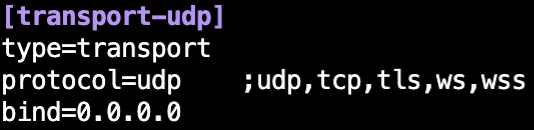
\includegraphics[width=0.6\textwidth]{img/pjsip.png}
		\caption{Configuration de pjsip.conf}
		\label{fig:pjsip}
	\end{figure}\\
	Ce sont des entrées de configuration pour la définition d'un transport 
	PJSIP dans le fichier de configuration d'Asterisk.
	\begin{itemize}
		\item \textbf{[transport-udp]} définit un nom pour le transport, "transport-udp" en l'occurrence.\\
		\item \textbf{type = transport} indique le type de l'objet de configuration. Ici, il s'agit d'un transport PJSIP.\\
		\item \textbf{protocol = udp} définit le protocole de transport utilisé, en l'occurrence l'UDP (User Datagram Protocol).\\
		\item \textbf{bind = 0.0.0.0} définit l'interface réseau sur laquelle le transport écoutera les connexions. La valeur "0.0.0.0" signifie que le transport écoutera sur toutes les interfaces disponibles.\\
	\end{itemize}

	\newpage 
	

	Puis, \textbf{pjsip wizard.conf} :
	\begin{figure}[h]
		\centering
		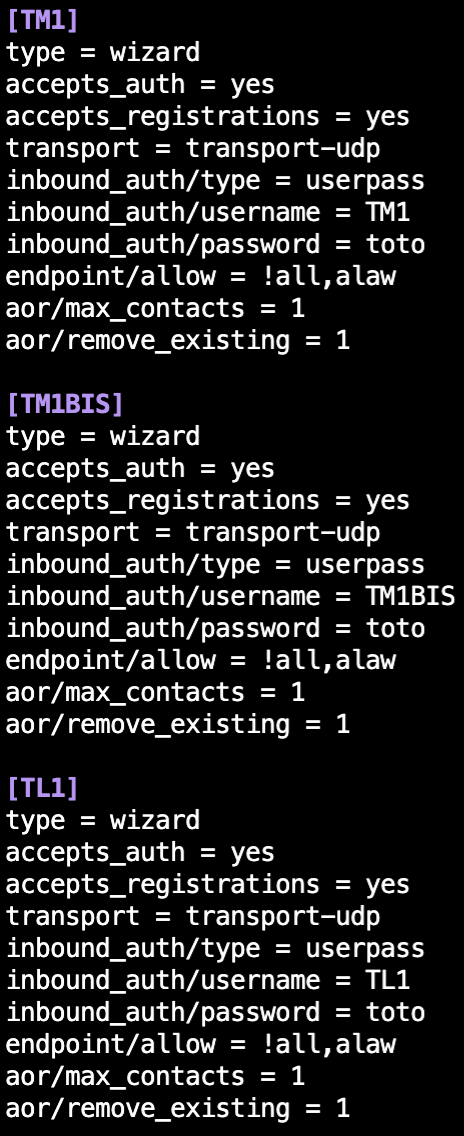
\includegraphics[width=0.4\textwidth]{img/wizard.png}
		\caption{Configuration de pjsip wizard.conf}
		\label{fig:wiz}
	\end{figure}\\

	Nous avons ici donc la configuration de tous les téléphones. A chaque fois, j'ai
	donc déclaré un téléphone avec son numéro de téléphone, son mot de passe et son
	nom d'utilisateur. Certaines lignes permettent de faire différentes choses
	essentielles au bon fonctionnement du serveur Asterisk, je vais détailler 
	toutes les explications à la page suivante. 

	\subsubsection*{Explication des lignes de configuration}
	Je vais prendre pour exemple l'utilisateur \textbf{[TL1]} car c'est après
	assez similaire pour les autres déclarations d'utilisateurs. 

	\begin{itemize}
		\item \textbf{[TL1]} : définit un nom pour l'endpoint, "TL1" en l'occurrence.\\
		\item \textbf{accepts\_auth = yes} et \textbf{accepts\_registrations = yes} autorisent l'authentification et l'enregistrement des utilisateurs pour cet endpoint.\\
		\item \textbf{transport = transport-udp} définit le transport PJSIP à utiliser pour acheminer les appels à travers le réseau pour cet endpoint.\\
		\item \textbf{inbound\_auth/type = userpass} définit le type d'authentification pour les appels entrants à cet endpoint, en l'occurrence l'authentification par nom d'utilisateur et mot de passe.\\
		\item \textbf{inbound\_auth/username = TL1} et \textbf{inbound\_auth/password = toto} définissent le nom d'utilisateur et le mot de passe pour l'authentification.\\
		\item \textbf{endpoint/allow = !all,alaw} définit les codecs audio autorisés pour les appels entrant et sortant à partir de cet endpoint. \textbf{alaw} est un codec audio couramment utilisé et \textbf{!all} signifie que tous les autres codecs ne sont pas autorisés.\\
		\item \textbf{aor/max\_contacts = 1} et \textbf{aor/remove\_existing = 1} définissent les paramètres de gestion des connexions pour cet endpoint. \textbf{Aor/max\_contacts = 1} signifie qu'un seul contact peut être enregistré pour cet endpoint à tout moment, tandis que \textbf{aor/remove\_existing = 1} signifie que les connexions existantes seront supprimées lorsqu'une nouvelle connexion est établie.\\
		\item \textbf{endpoint/call\_group = 1} et \textbf{endpoint/pickup\_group = 1} définissent les groupes d'appels et de prise en charge pour cet endpoint. Les numéros d'identification des groupes peuvent varier selon votre configuration.\\
	\end{itemize}


	Un \textbf{endpoint} est peut être un téléphone IP, un softphone, 
	une interface de téléphonie sur un ordinateur, ou tout autre appareil 
	capable de communiquer avec le système de téléphonie Asterisk.
	
	\newpage
	\subsubsection{Pour le service IPBX, créer le plan de numérotation}
	J'ai donc crée le plan de numérotation de la même manière que nous l'avons vu en cours
	et en TP comme peut en témoigner la capture d'écran suivante en rajoutant bien 
	entendu ces lignes dans le contexte \texttt{[default]} :
	\begin{figure}[h]
		\centering
		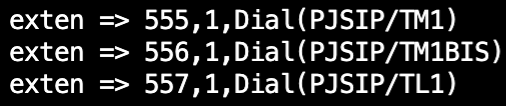
\includegraphics[width=0.7\textwidth]{img/extensions.png}
		\caption{Configuration de extensions.conf}
		\label{fig:ext}
	\end{figure}\\
	J'ai choisi de réutiliser dans un premier temps les numéros que l'on utilisait
	en cours pour me faciliter la compréhension. Ce sont des numéros, que j'ai à terme 
	modifié en 1, 2 et 3.\\

	\textbf{Exten => 555,1} définit le numéro de l'extension à 555. Lorsqu'un 
	appel est effectué à cet extension, les instructions suivantes seront 
	exécutées. \textbf{Dial(PJSIP/TM1)} est l'instruction pour composer un 
	appel. \textbf{Dial} est une commande intégrée d'Asterisk qui permet de 
	composer un appel vers une destination donnée. \textbf{PJSIP/TM1} est la 
	destination de l'appel.
	
	\textbf{PJSIP} désigne le protocole de téléphonie IP utilisé 
	(dans ce cas, PJSIP) et \textbf{TM1} est le nom de l'endpoint ou 
	de l'utilisateur auquel l'appel doit être dirigé.

\subsection{Configuration Téléphone Clients}
	\subsubsection{Téléphone logiciel Linphone}
	Tout d'abord j'ai voulu configurer linphone sur la machine windows de l'IUT
	sur laquelle j'ai fait ma VM Debian. Cependant, j'ai eu de nombreux problèmes
	Linphone ne fonctionnait pas, même après avoir essayé plusieurs versions. 
	J'ai donc essayé d'utiliser mon ordinateur personnel pour faire cette 
	manipulation. J'ai donc installé Linphone sur mon ordinateur personnel et 
	ça a fonctionné. Pour faire marcher Linphone j'ai utilisé la configuration suivante : \textit{Où 10.129.10.164 est l'IP de mon serveur Asterisk}
	\begin{figure}[h]
		\centering
		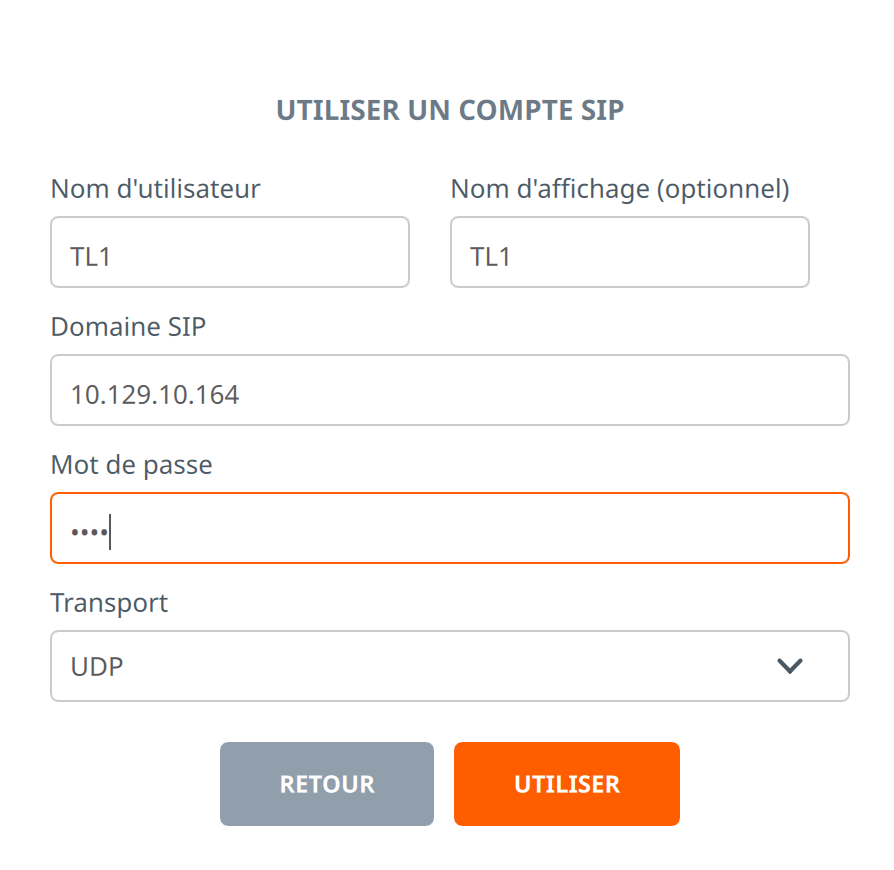
\includegraphics[width=0.5\textwidth]{img/linphone.png}
		\caption{Configuration de Linphone}
		\label{fig:lin}
	\end{figure}\\

	\subsubsection{Téléphone matériel Nortel LIP6812}
	\subsubsection*{Inscrivez le téléphone auprès du registrar de l'IPBX}
	Pour enregistrer le téléphone IP LG Nortel auprès du serveur IPBX, j'ai du
	le configurer directement depuis son interface pour rentrer tous les paramètres 
	pour qu'il puisse se connecter. \\
	Voici les différents paramètres que j'ai dû configurer pour que le téléphone remonte :
	J'ai du rentrer dans les paramètres du téléphone en appuyant sur la touche 
	\textbf{settings}, puis choisir le sous menu 2. \textbf{SIP configuration}
	\begin{figure}[h]
		\centering
		\rotatebox{-90}{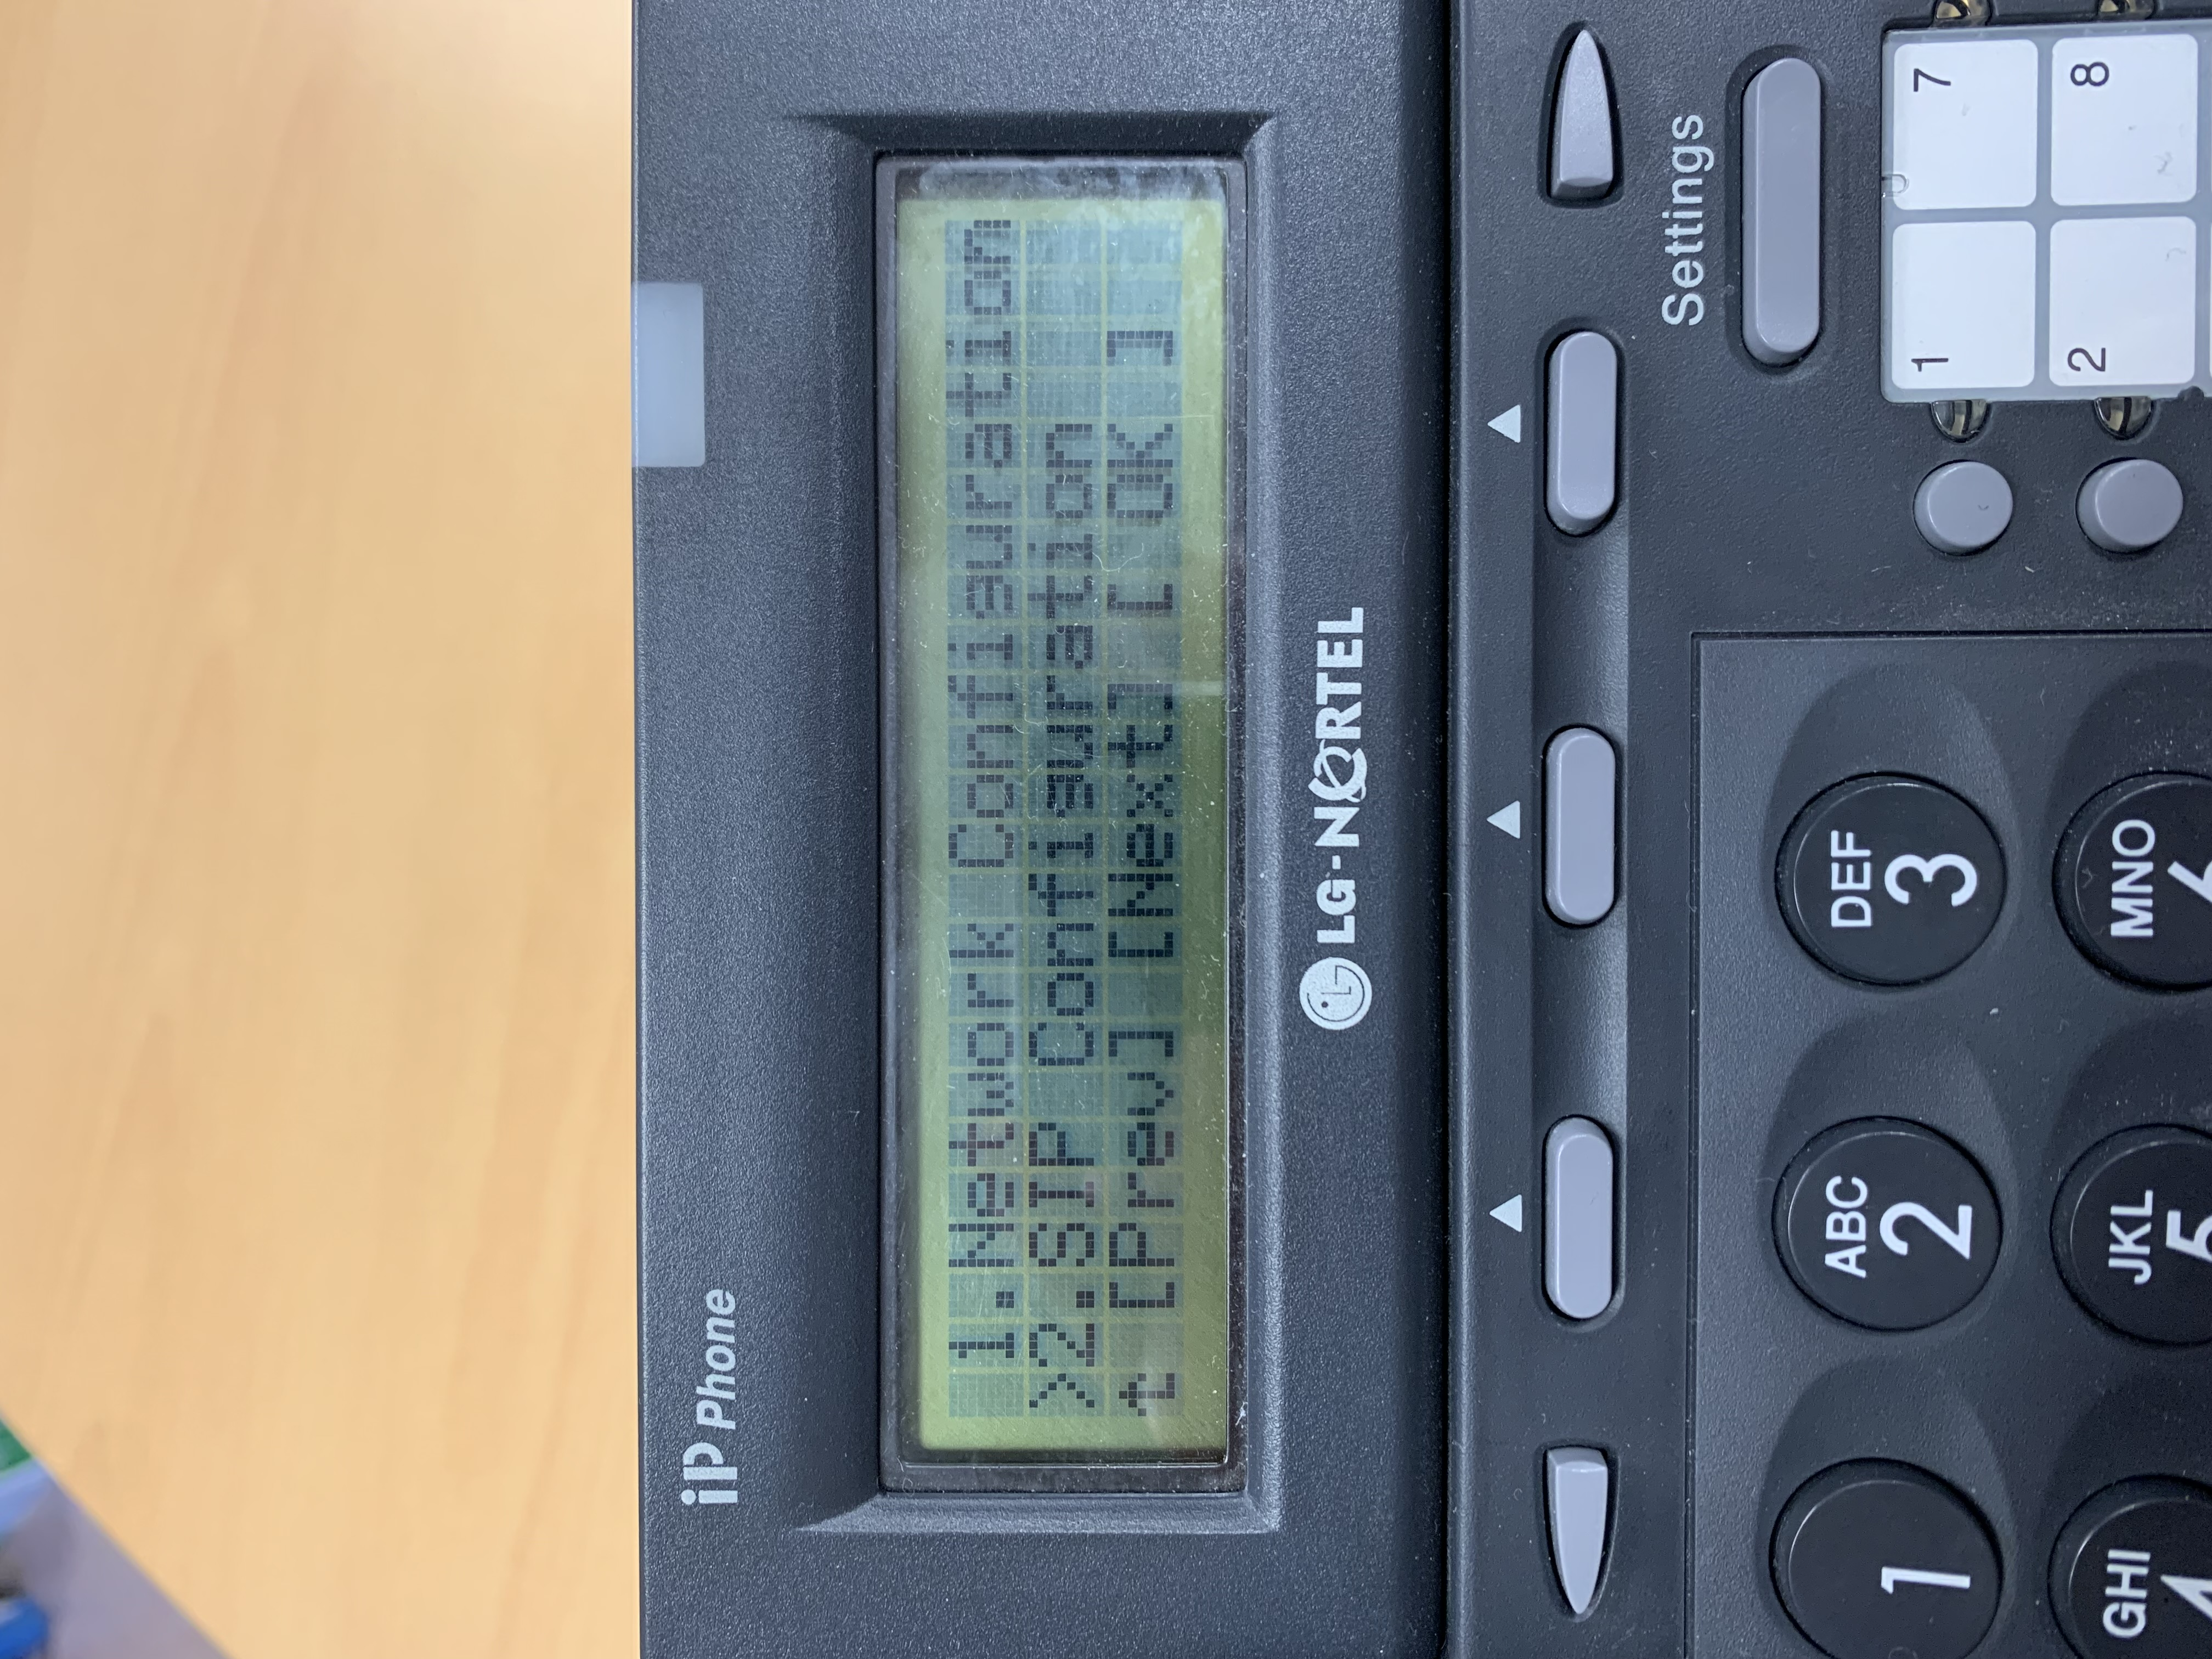
\includegraphics[width=0.4\textwidth]{img/IMG_0512.jpeg}}
		\caption{Choix menu SIP configuration}
		\label{fig:set}
	\end{figure}\\
	Ensuite, je viens sélectionner la ligne 1. \textbf{Line 1 Settings}
	\begin{figure}[h]
		\centering
		\rotatebox{-90}{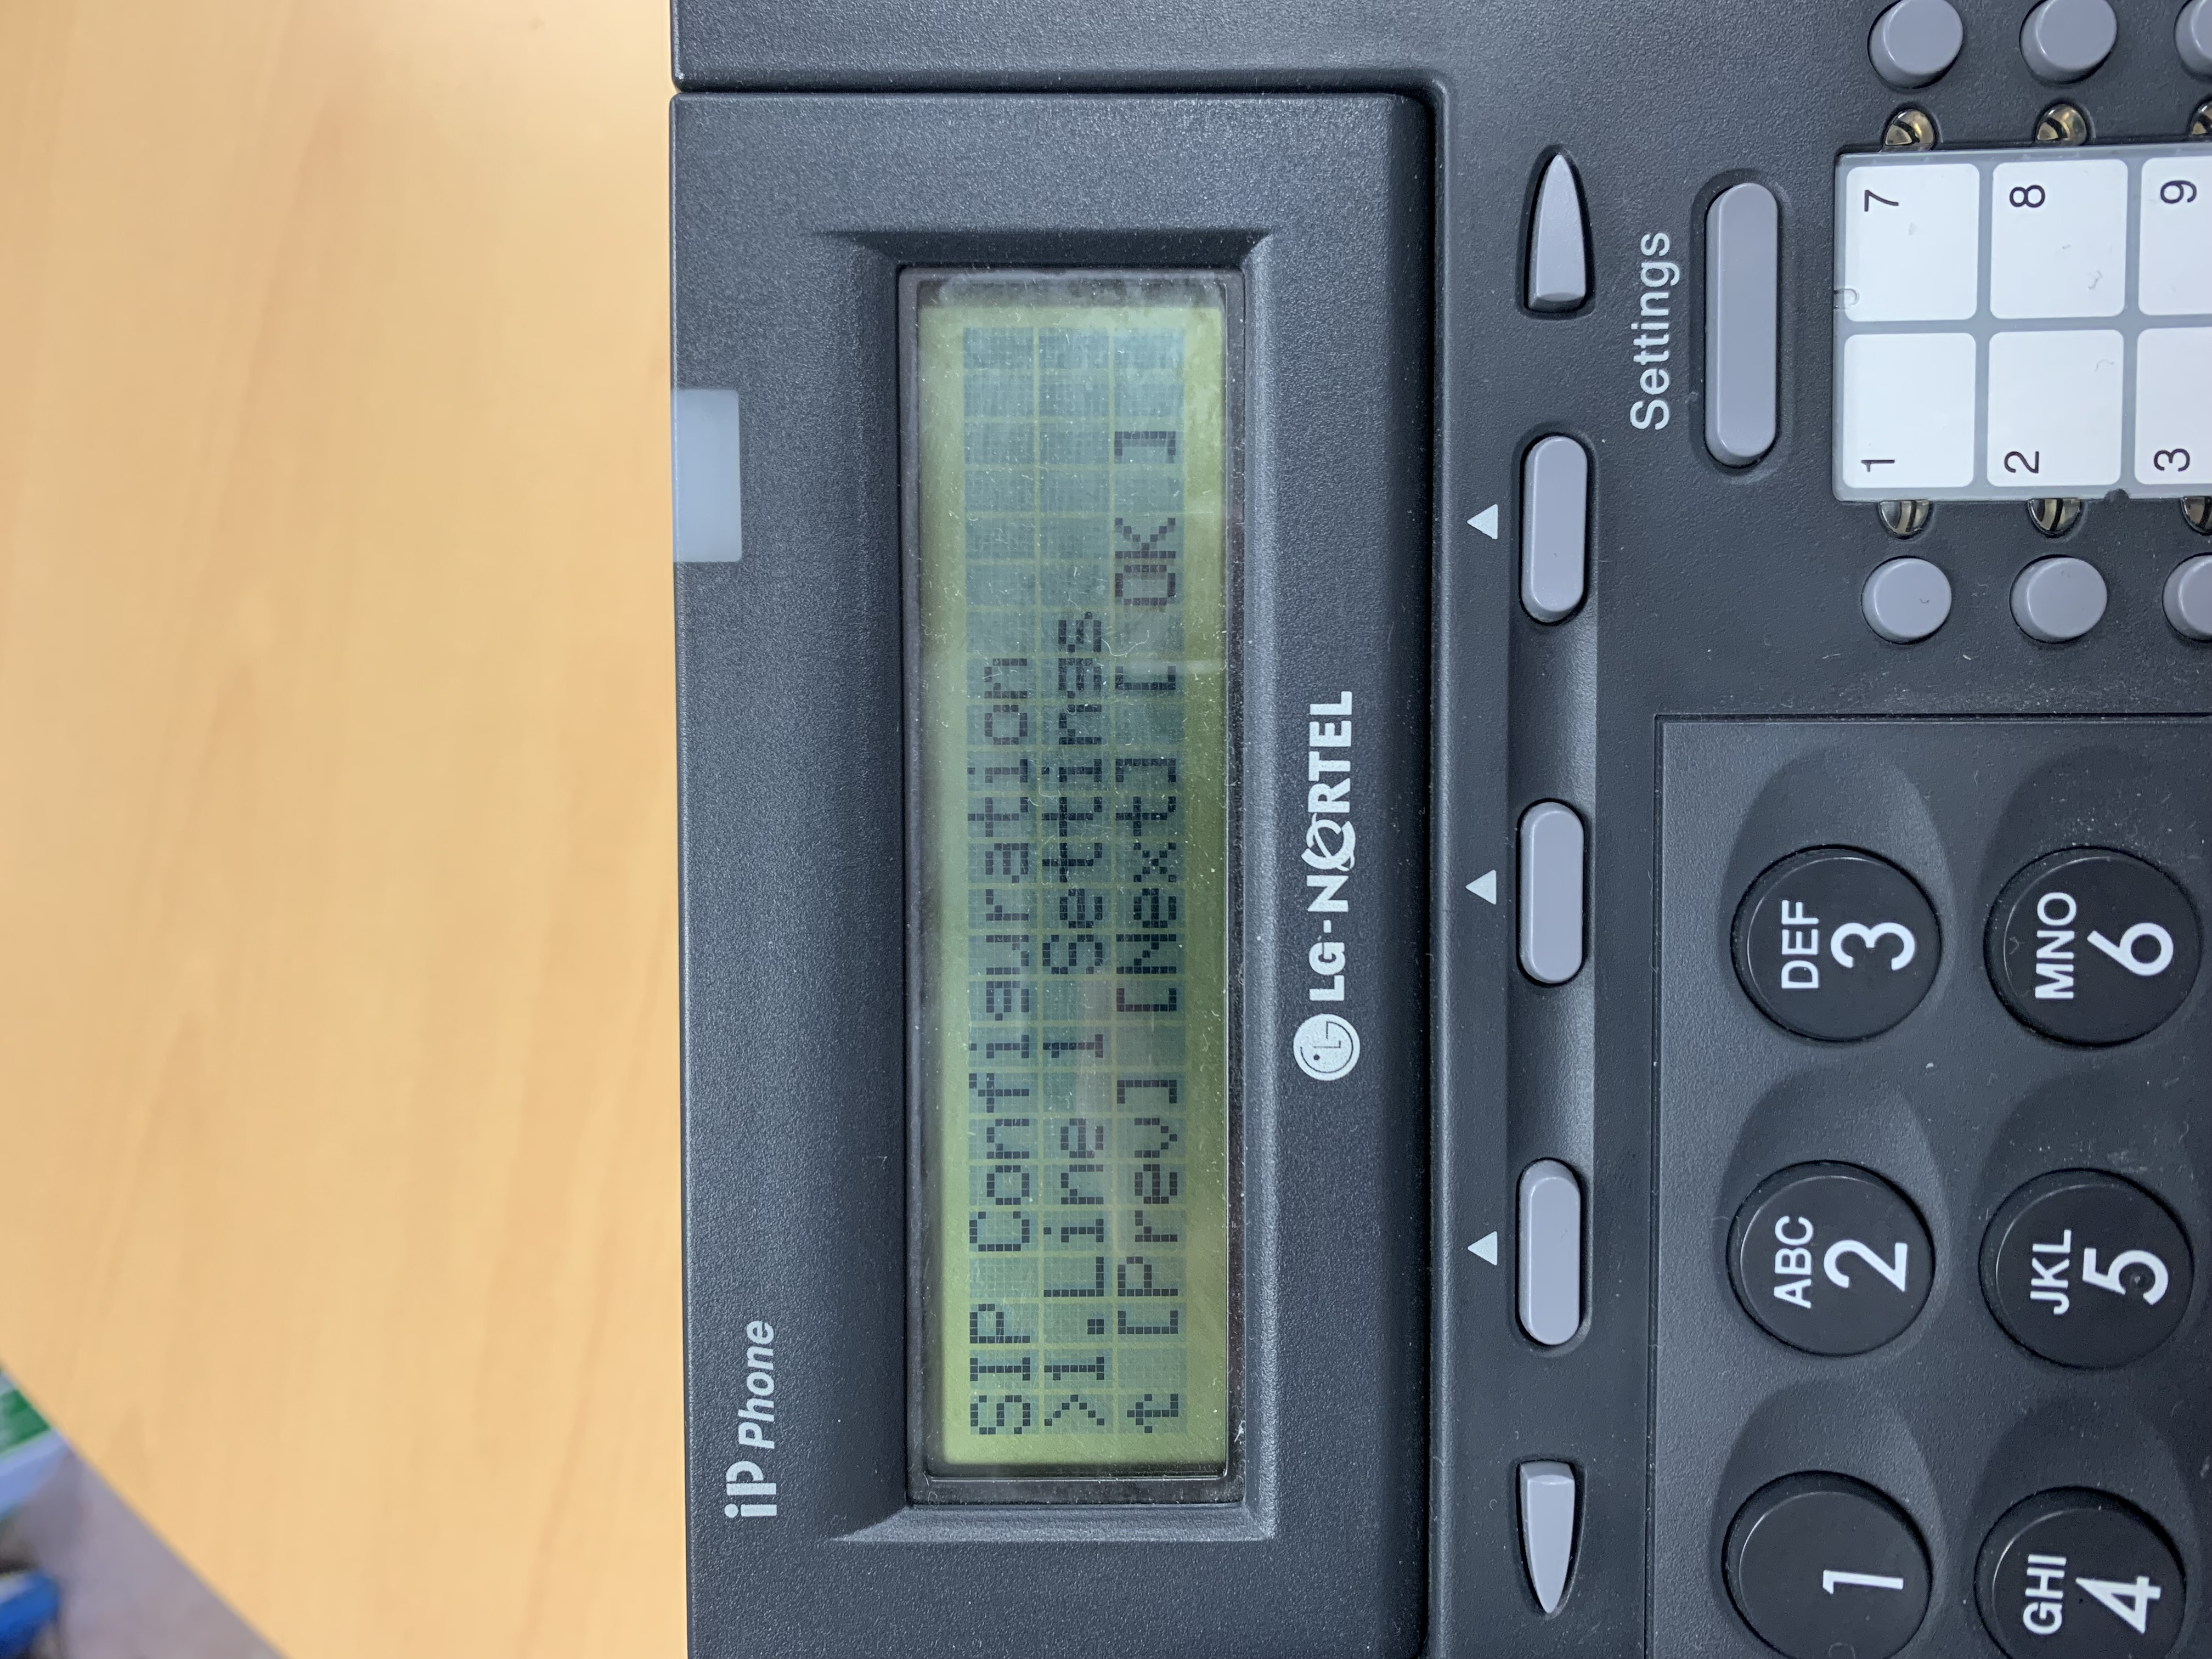
\includegraphics[width=0.4\textwidth]{img/IMG_0513.jpeg}}
		\caption{Choix menu Line 1 settings}
		\label{fig:set}
	\end{figure}\\
	Pour finir, je viens configurer l'ensemble des paramètes qui sont inscrits
	comme par exemple, l'adresse IP du serveur IPBX, le nom d'utilisateur,
	le mot de passe ainsi de suite...\\
	\begin{figure}[h]
		\centering
		\rotatebox{-90}{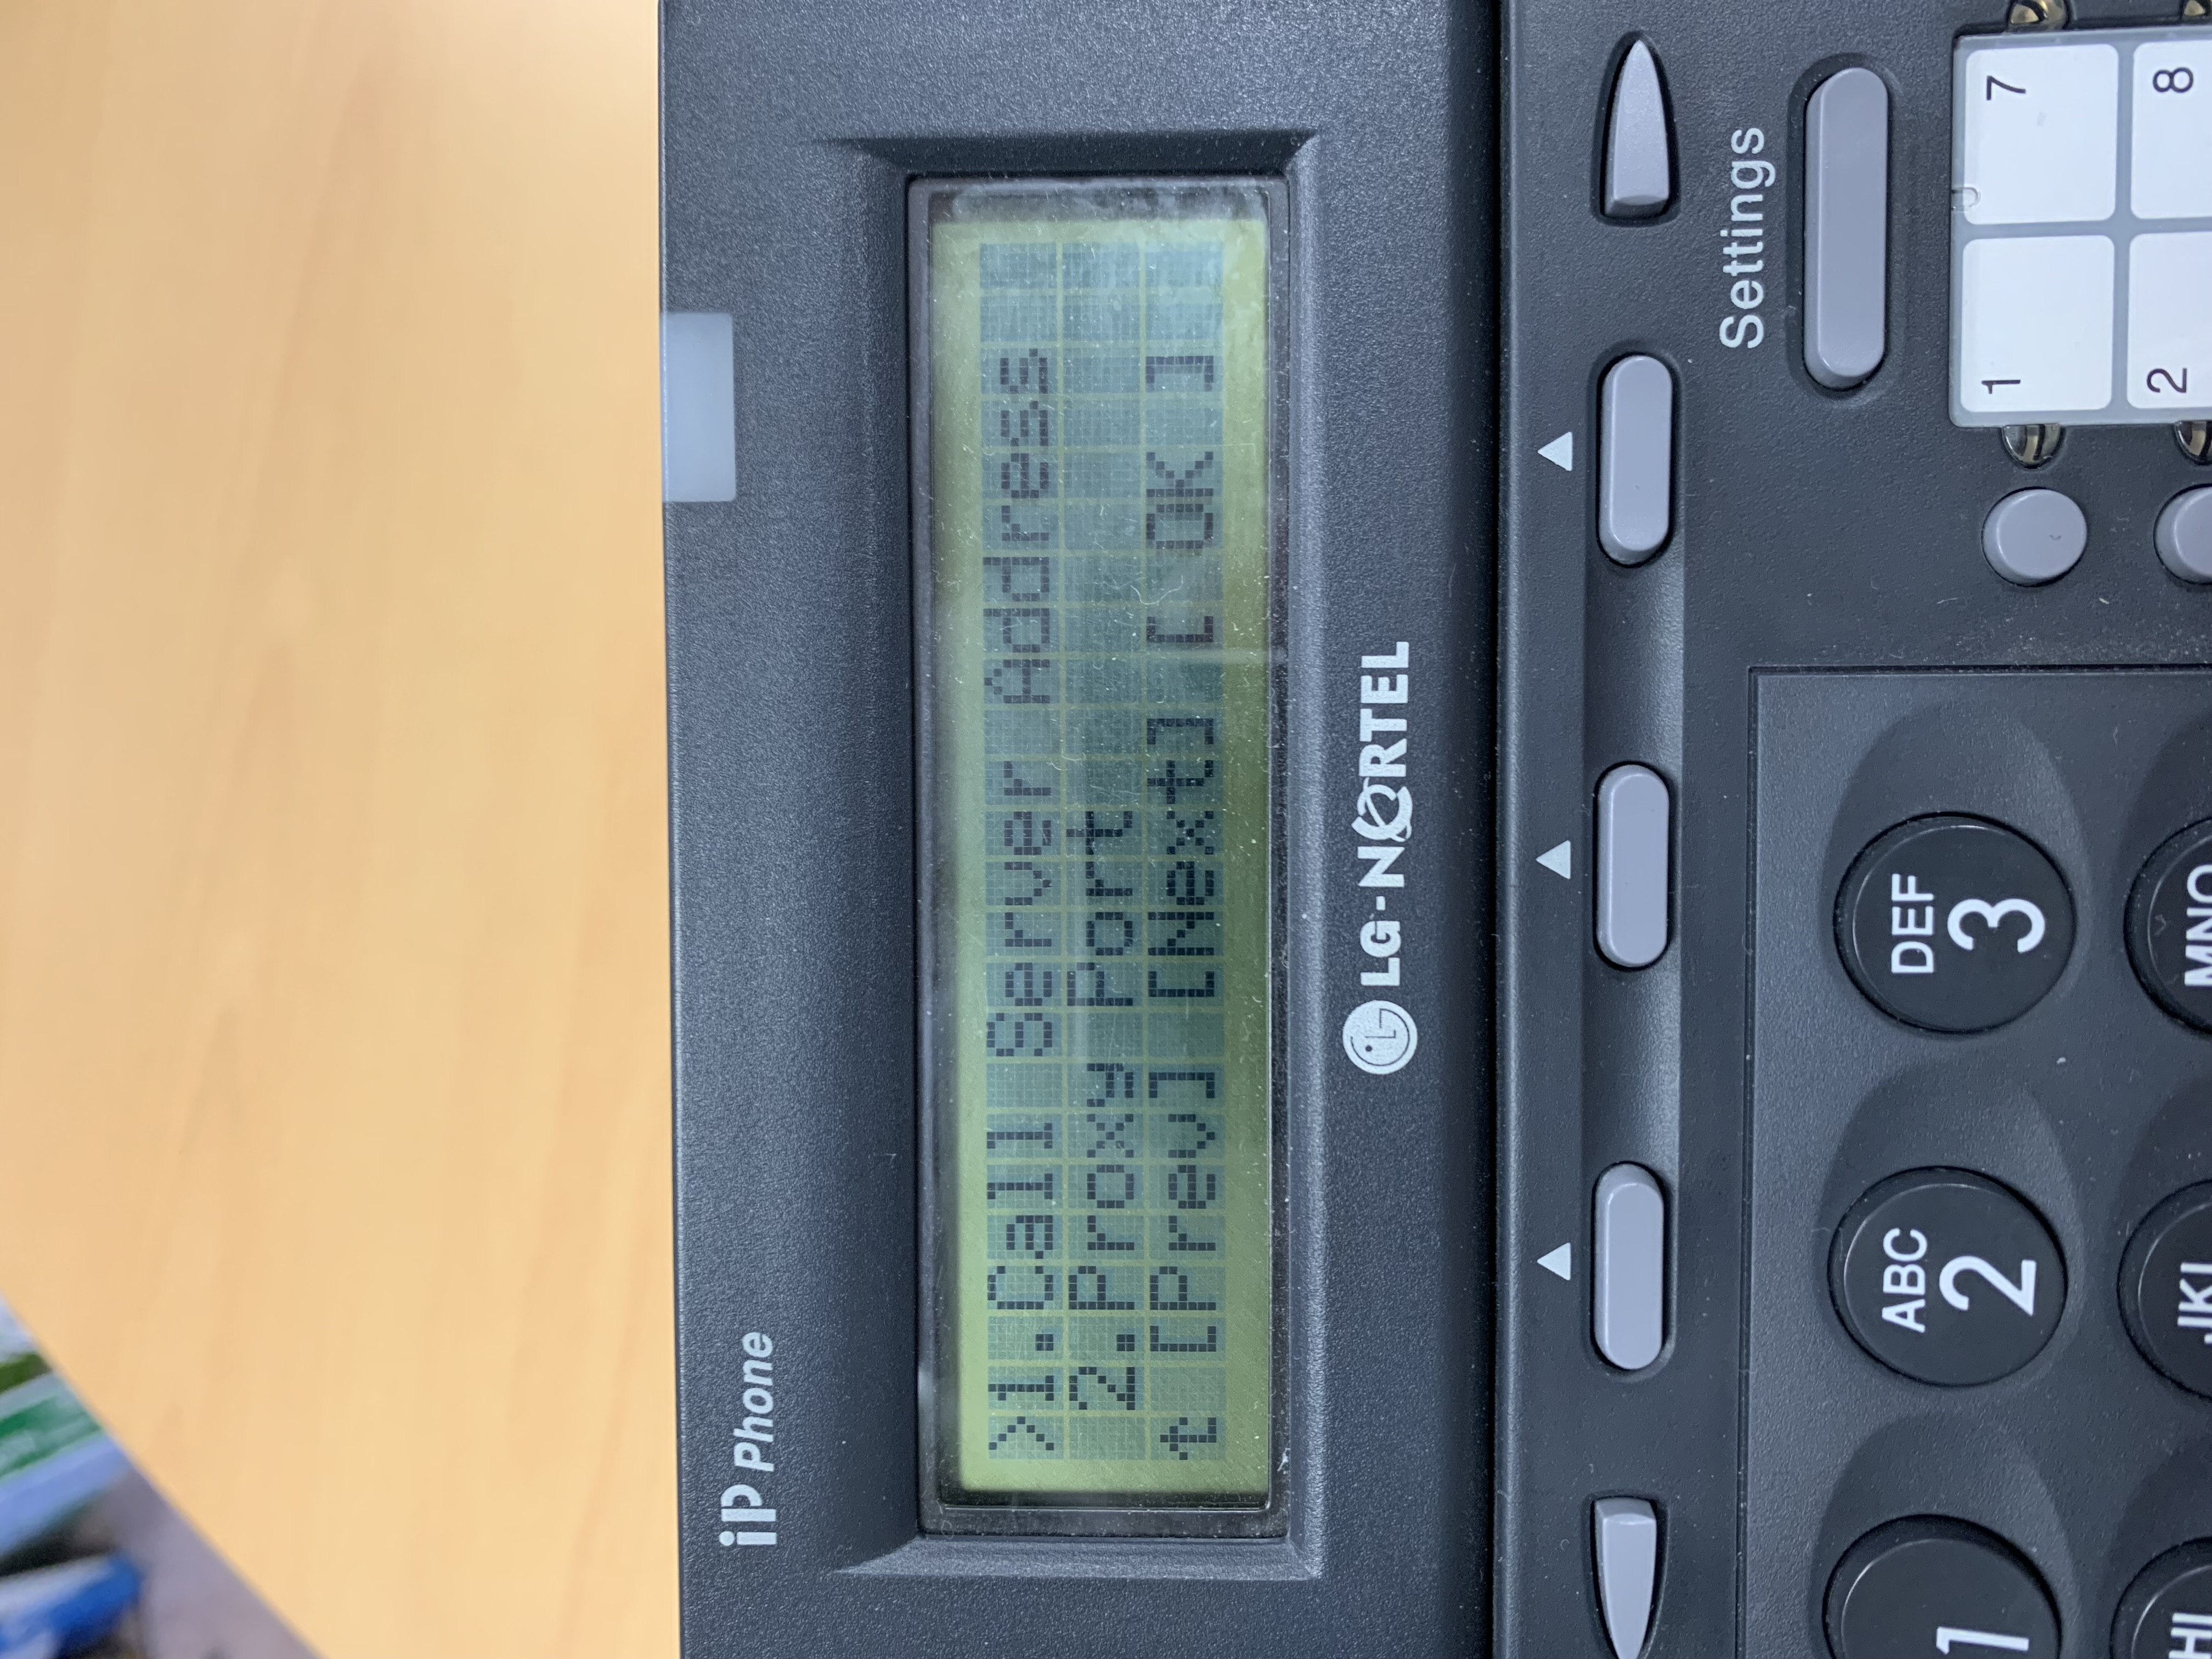
\includegraphics[width=0.4\textwidth]{img/IMG_0514.jpeg}}
		\caption{Configuration du Nortel}
		\label{fig:set}
	\end{figure}\\
	Une fois configuré correctement le téléphone remonte automatiquement auprès
	du serveur IPBX et nous pouvons l'utiliser pour appeler en interne. 


	\subsubsection{Téléphone Matériel Cisco 7941G}
	\subsubsection*{Etudiez la procédure d'installation d'un nouveau firmware}
	Pour installer un nouveau firmware sur le Cisco 7941G. Il a d'abord fallu 
	monter un serveur TFTP afin de pouvoir envoyer le firmware sur le téléphone.
	Nous avons donc monter un serveur TFTP à l'aide de mes camarades, sur windows comme
	le démontre la photo qui suit : 
	
	\begin{figure}[h]
		\centering
		{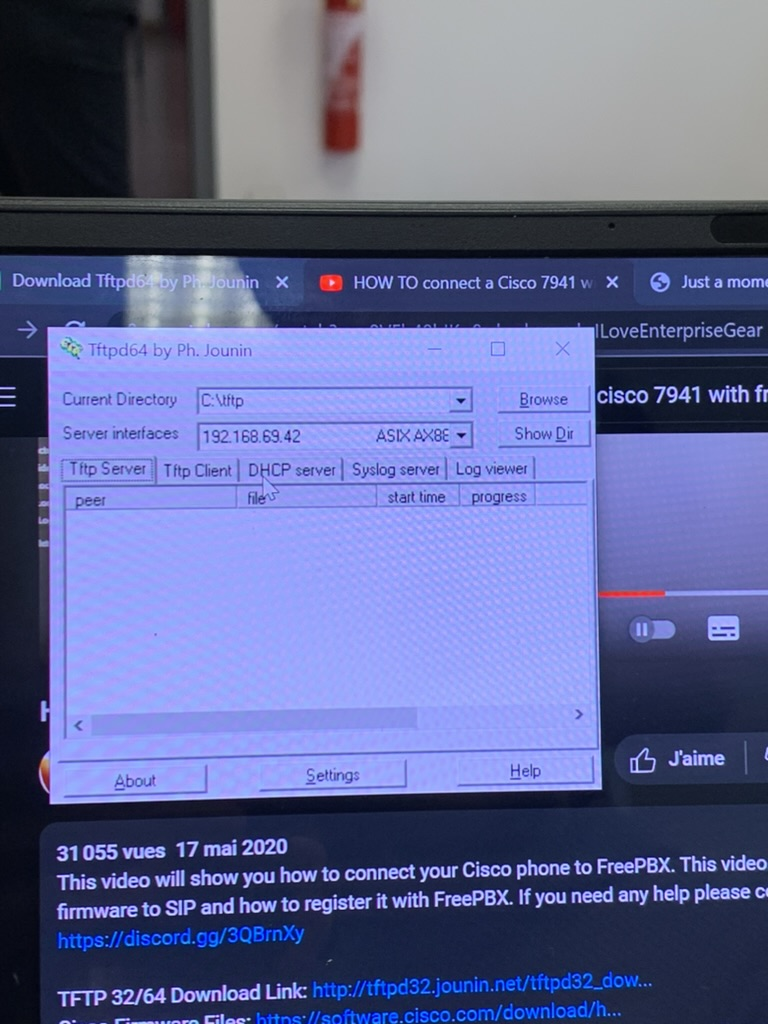
\includegraphics[width=0.6\textwidth]{img/85DFF5EE-EF97-4E83-9172-4FDA03718B73_1_105_c.jpeg}}
		\caption{Configuration du serveur TFTP}
		\label{fig:tftp}
	\end{figure}
	
	Puis, nous avons envoyer la configuration dans les téléphones. 
	L'envoie du nouveau firmware a donc bel et bien fonctionné. Cependant,
	nous avons eu des problèmes pour configurer le téléphone pour pouvoir
	l'enregistrer auprès du serveur Astetisk. Etant bloqués par la configuration
	du téléphone. Nous n'avons pas réussi à l'enregistrer. Même après avoir
	essayé de différentes manières, comme en essayant plusieurs firmwares.\\ 


	Comme nous pouvons le constater sur le photo qui suit, nous avons bien
	réussi à flasher les téléphones. Pour pouvoir les tenir prêt au flash
	il a fallu maintenir le bouton "\#" pendant le démarrage du téléphone. 
	Une fois que les boutons de volumes commençaient à clignoter il a fallu
	faire succéder les touches suivantes : \textbf{1, 2, 3, 4, 5, 6, 7, 8, 9, 0}
	Et, nous rentrions dans le mode de flashage comme le montre la photo qui suit : 
	\begin{figure}[h]
		\centering
		{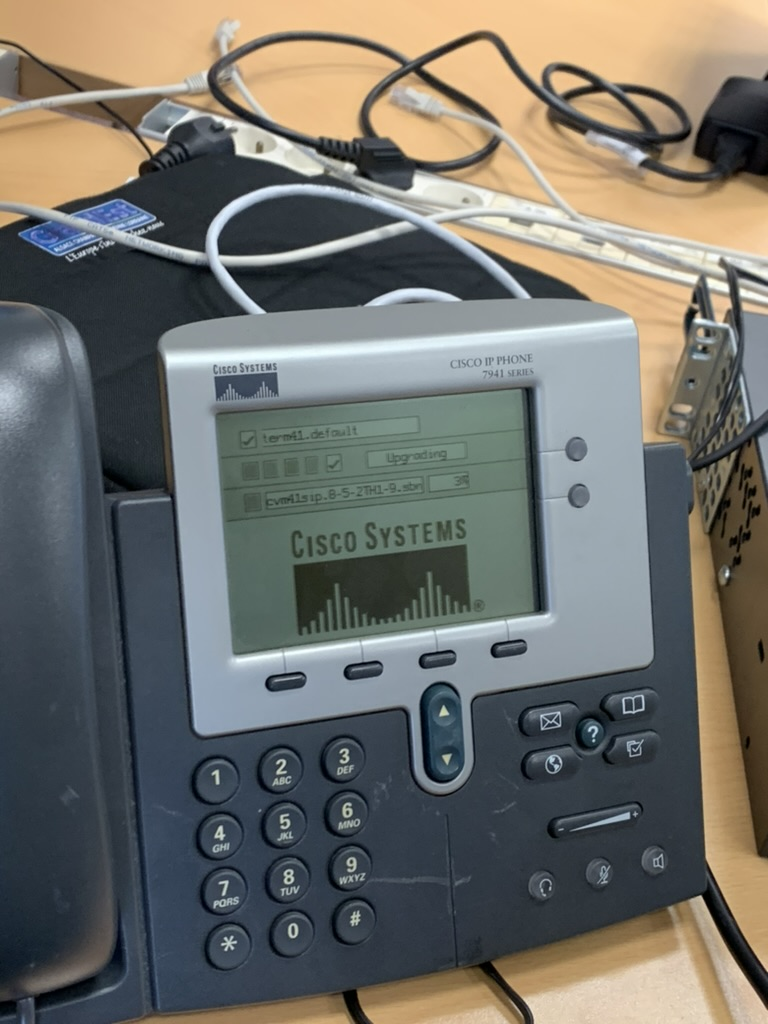
\includegraphics[width=0.6\textwidth]{img/F316F6A2-F9B9-4515-9004-3596AD28EBC8_1_105_c.jpeg}}
		\caption{Entrée du téléphone en mode flash}
		\label{fig:flash}
	\end{figure}

\subsection{Validation des appels}
Nous avons donc testé les différents appels internes possibles, et tout 
est fonctionnel, j'arrive bien à joindre la secrétaire, depuis le 
softphone et inversenement. 

\newpage
\section{Objectif 2 : Configuration inter-sites}
	\subsection{Appels inter-sites}
	\subsubsection{Sur l'IPBX, inscrire le faiceau SIP}
	Pour inscrire mon faisceau SIP auprès de l'opérateur Voix, j'ai 
	configuré un nouveau contexte \textbf{[operateurvoix]} et que j'ai configuré
	comme ci-arpès : 

	\begin{figure}[h]
		\centering
		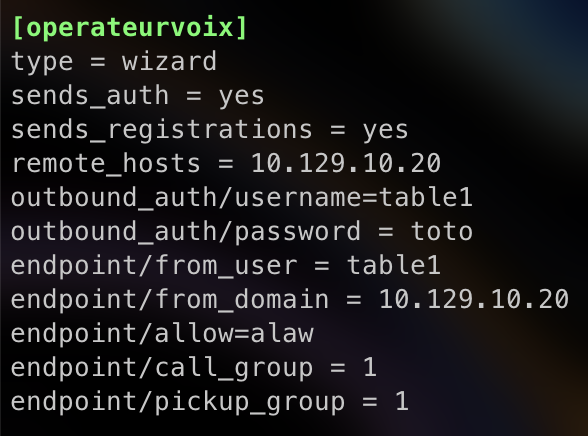
\includegraphics[width=0.4\textwidth]{img/inter.png}
		\caption{Configuration de l'opérateur Voix}
		\label{fig:opvoix}
	\end{figure}
	Je définis à chaque fois les bons paramètres que je vais expliquer ci-après :
	\begin{itemize}
		\item \texttt{remote\_hosts} : Définis l'adresse IP du serveur Opérateur Voix
		\item \texttt{outbound\_auth} : Définis le nom d'utilisateur et le mot de passe pour communiquer à travers le serveur voix
	\end{itemize}


	\subsubsection{Dans le plan de numérotation, ajoutez le préfix *}
	Dans mon fichier \textbf{extensions.conf}, j'ai donc rajouté la ligne suivante
	dans le contexte \textbf{[default]} :
	\begin{figure}[h]
		\centering
		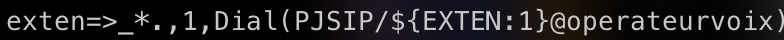
\includegraphics[width=0.7\textwidth]{img/exten-op.png}
		\caption{Configuration de l'opérateur voix dans extensions.conf}
		\label{fig:op-ext}
	\end{figure}\\
	\begin{itemize}
		\item \textbf{exten => \_.,1} signifie que cette extension est associée à tout numéro composé, quelle que soit la longueur et les chiffres qui le composent. Le "" signifie n'importe quel nombre et le "." signifie n'importe quelle longueur.
		\item \textbf{Dial(PJSIP/\${EXTEN:1}@operateurvoix)} signifie que l'appel sera acheminé via le protocole PJSIP en utilisant l'opérateur de voix défini. La variable "\${EXTEN:1}" est utilisée pour extraire le numéro composé par l'utilisateur, en excluant le premier caractère qui est un "\_".
	\end{itemize}

	\subsubsection{Validez les appels entrants et sortants entre cabinets médicaux}
	Suite à la configuration de l'opérateur voix, j'ai pu tester les appels entrants et sortants entre les différents
	cabinets de mes camarades. Tout est fonctionnel. Si par exemple je veux joindre
	Victor Uetwiller à la table7. Je compose \texttt{**72} et j'arrive bien
	à l'appeler. 

	\subsection{Appels externes}
	\subsubsection{Ajoutez les numéros à 10 chiffres pour les appels extérieurs via le faisceau}
	Pour pouvoir appeler à l'éxterieur de mon faisceau les appels à 10 chiffres, j'ai ajouté la ligne
	suivante dans le fichier \textbf{extensions.conf} :
	\begin{figure}[h]
		\centering
		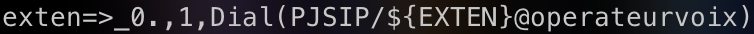
\includegraphics[width=0.7\textwidth]{img/externes.png}
		\caption{Configuration des appels à 10 chiffres extensions.conf}
		\label{fig:exter}
	\end{figure}\\

	\begin{itemize}
		\item \textbf{exten=>\_0.,1} définit le numéro de l'extension avec un masque de correspondance général, où \textbf{\_0.} signifie que cette extension sera activée pour tout numéro de téléphone commençant par \textbf{0}.\\
		\item \textbf{Dial(PJSIP/\${EXTEN}@operateurvoix)} est l'instruction pour composer un appel. \textbf{Dial} est une commande intégrée d'Asterisk qui permet de composer un appel vers une destination donnée. \textbf{PJSIP/\${EXTEN}@operateurvoix} est la destination de l'appel. \textbf{PJSIP} désigne le protocole de téléphonie IP utilisé (dans ce cas, PJSIP) et \textbf{\${EXTEN}} est une variable qui contient le numéro d'appel entrant (sans le "0" initial). \textbf{Operateurvoix} est le nom d'un serveur ou d'un fournisseur de services de téléphonie IP auquel l'appel doit être dirigé.
	\end{itemize}

	\subsubsection{Validez les appels externes vers (0112345678)}
	J'ai donc testé d'appeler les appels vers le 0212345678, le numéro hébergé par
	Victor sur son PC. Et l'appel fonctionne parfaitement. 

\newpage
\section{Objectif 3 : Fonctions téléphoniques}
\subsection{Transfert d'appels}
	\subsubsection{Activez le transfert d'appels côté IPBX}
	Pour activer le transfert d'appels côté IPBX, j'ai donc modifié les lignes suivante 
	dans le fichier \textbf{extensions.conf} :
	\begin{figure}[h]
		\centering
		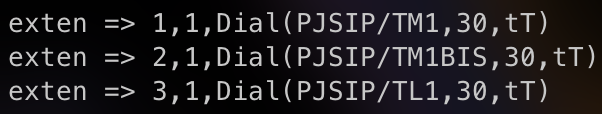
\includegraphics[width=0.7\textwidth]{img/tT.png}
		\caption{Configuration du transfert extensions.conf}
		\label{fig:trans}
	\end{figure}\\
	Il ne faut aussi pas oublier de décommenter la ligne \texttt{blindxfer => \#1}
	dans le fichier \textbf{features.conf} et dans le context \textbf{[featuremap]}.\\

	J'ai modifié le plan de numérotation des téléphones en ajoutant l'option
	\textbf{tT} pour le transfert d'appels. Désormais quand je suis en appel
	et que je compose la touche \textbf{\#1}, suivis du numéro de téléphone
	vers lequel je veux transférer l'appel et que je valide, l'appel est transféré.\\

	En utilisant les options \textbf{tT} dans la ligne de configuration, j'autorisez 
	les deux méthodes de transfert d'appel, soit en utilisant le code de 
	transfert ou en utilisant la touche de transfert rapide.

	\subsubsection{Validez le fonctionnement dans l'ensemble des cas possibles}
	Pour tester les transferts d'appel, j'ai tout d'abord testé en interne de 
	transférer mon appel vers un autre téléphone logiciel. Ce qui a fonctionné.
	Puis, pour compléxifier un peu le sujet, j'ai demandé à un camarade 
	de m'appeler. J'ai receptionné l'appel et j'ai transféré l'appel vers
	une autre table. Ce qui a également fonctionné.\\

	\newpage
	\subsubsection{Pour chaque téléphone, définissez un numéro de transfert}
	Pour définir une touche rapide de transfert sur le LG Nortel. Je suis 
	rentrer dans les paramètes, puis, j'ai cliqué sur le bouton numéro 
	3 qui correspond à \textbf{Phone settings} : 
	\begin{figure}[h]
		\centering
		\rotatebox{-90}{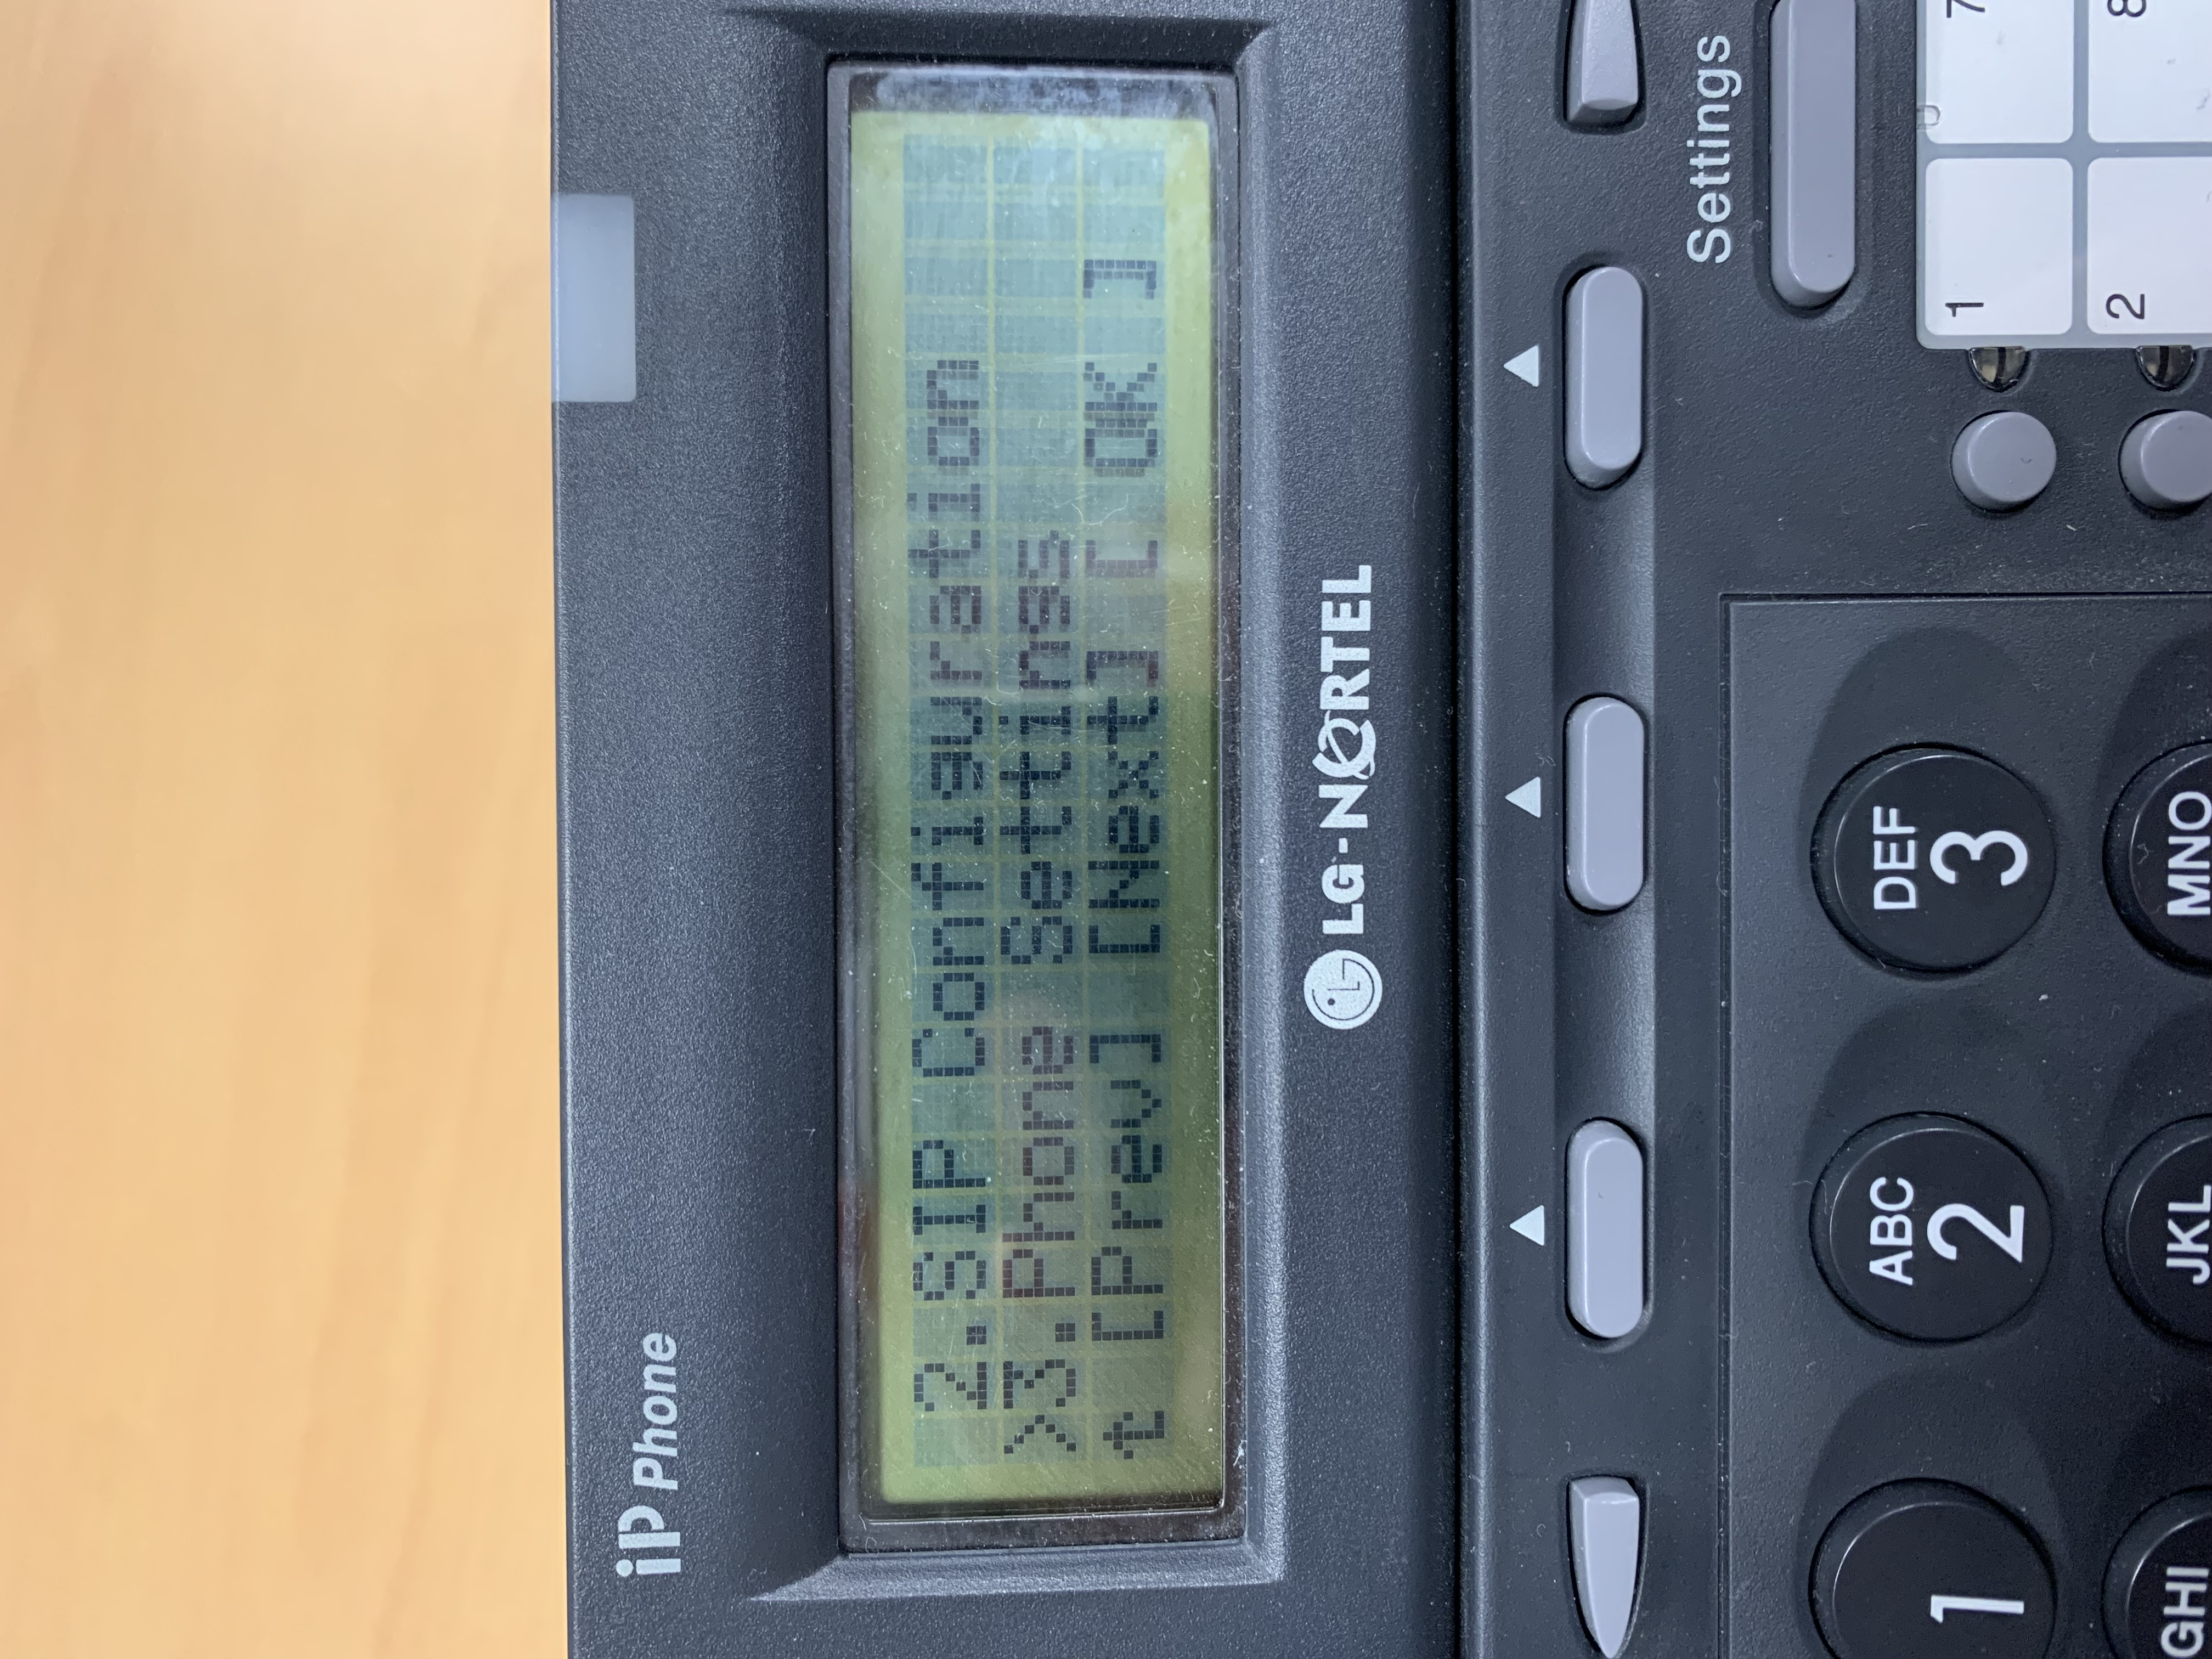
\includegraphics[width=0.4\textwidth]{img/IMG_0508.jpeg}}
		\caption{Phone settings}
		\label{fig:btnt}
	\end{figure}\\
	Puis, je me suis rendu dans le sous-menu 6, qui correspond à 
	\textbf{Flexible Key Settings} : 
	\begin{figure}[h]
		\centering
		\rotatebox{-90}{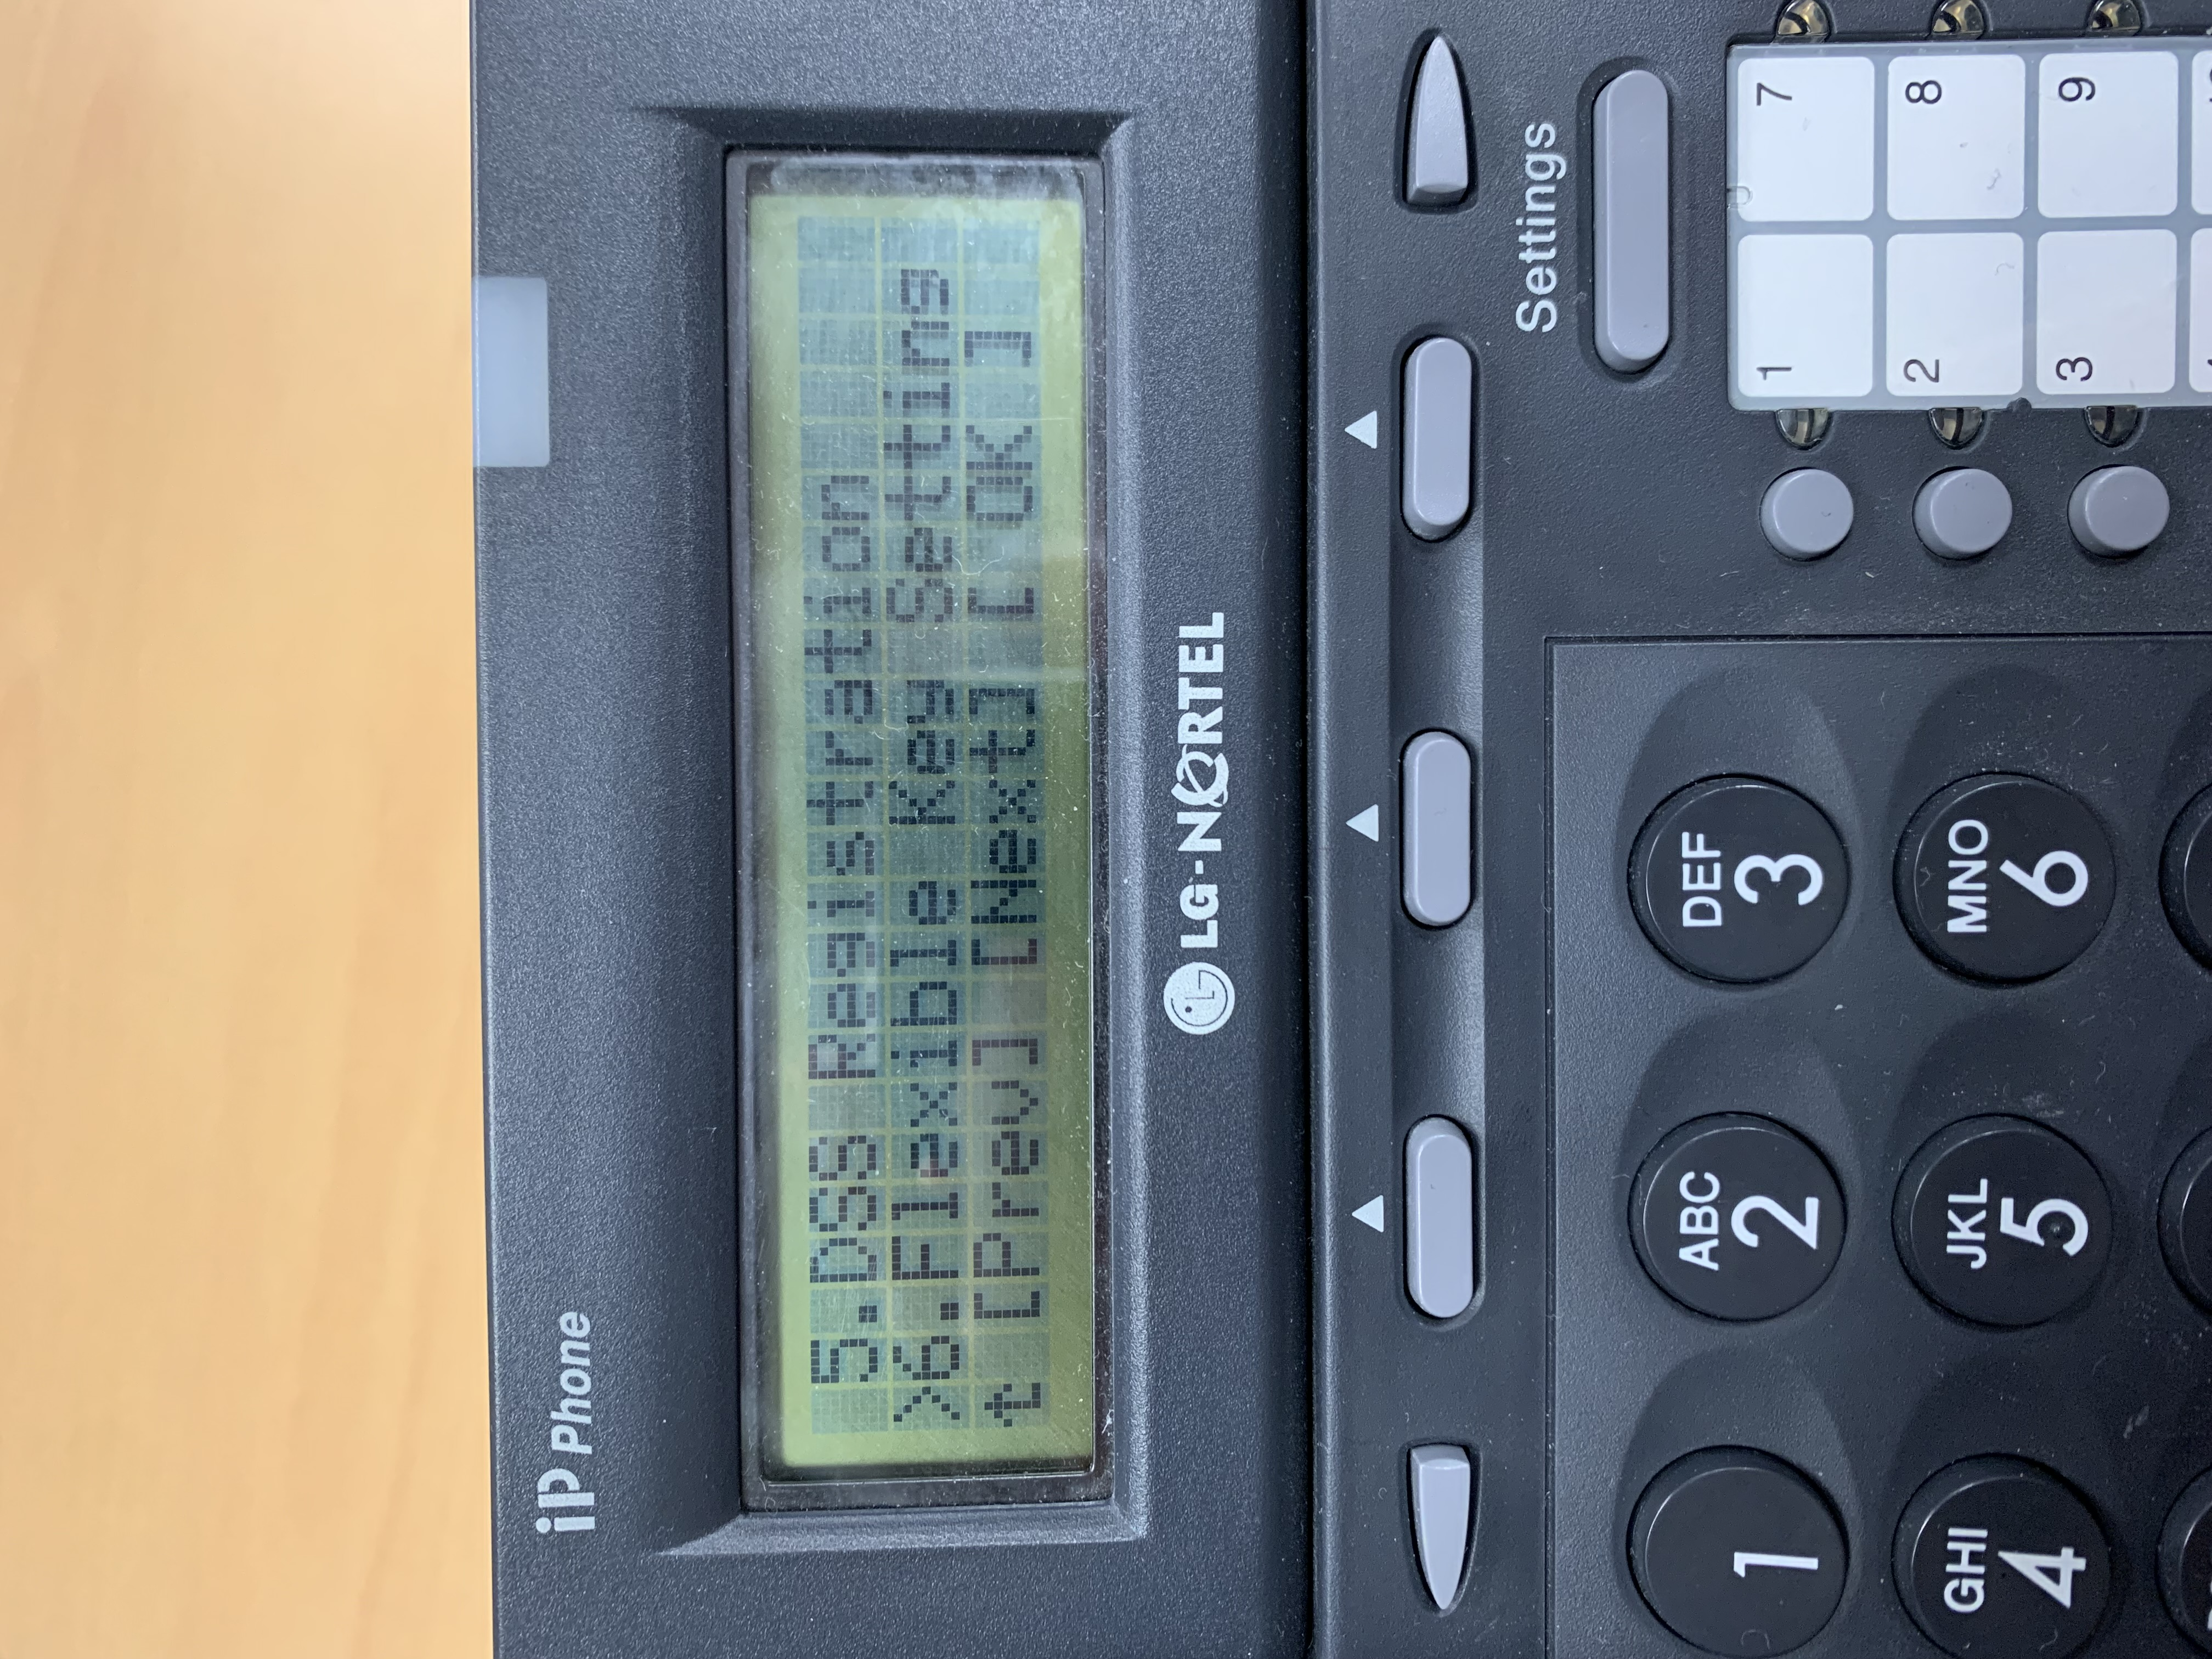
\includegraphics[width=0.4\textwidth]{img/IMG_0509.jpeg}}
		\caption{Flexible Key Settings}
		\label{fig:btnk}
	\end{figure}\\[2cm]

	J'ai ensuite choisi sur la touche que je voulais attribuer à ce raccourci
	en cliquant sur la touche que je souhaitais :
	\begin{figure}[h]
		\centering
		\rotatebox{-90}{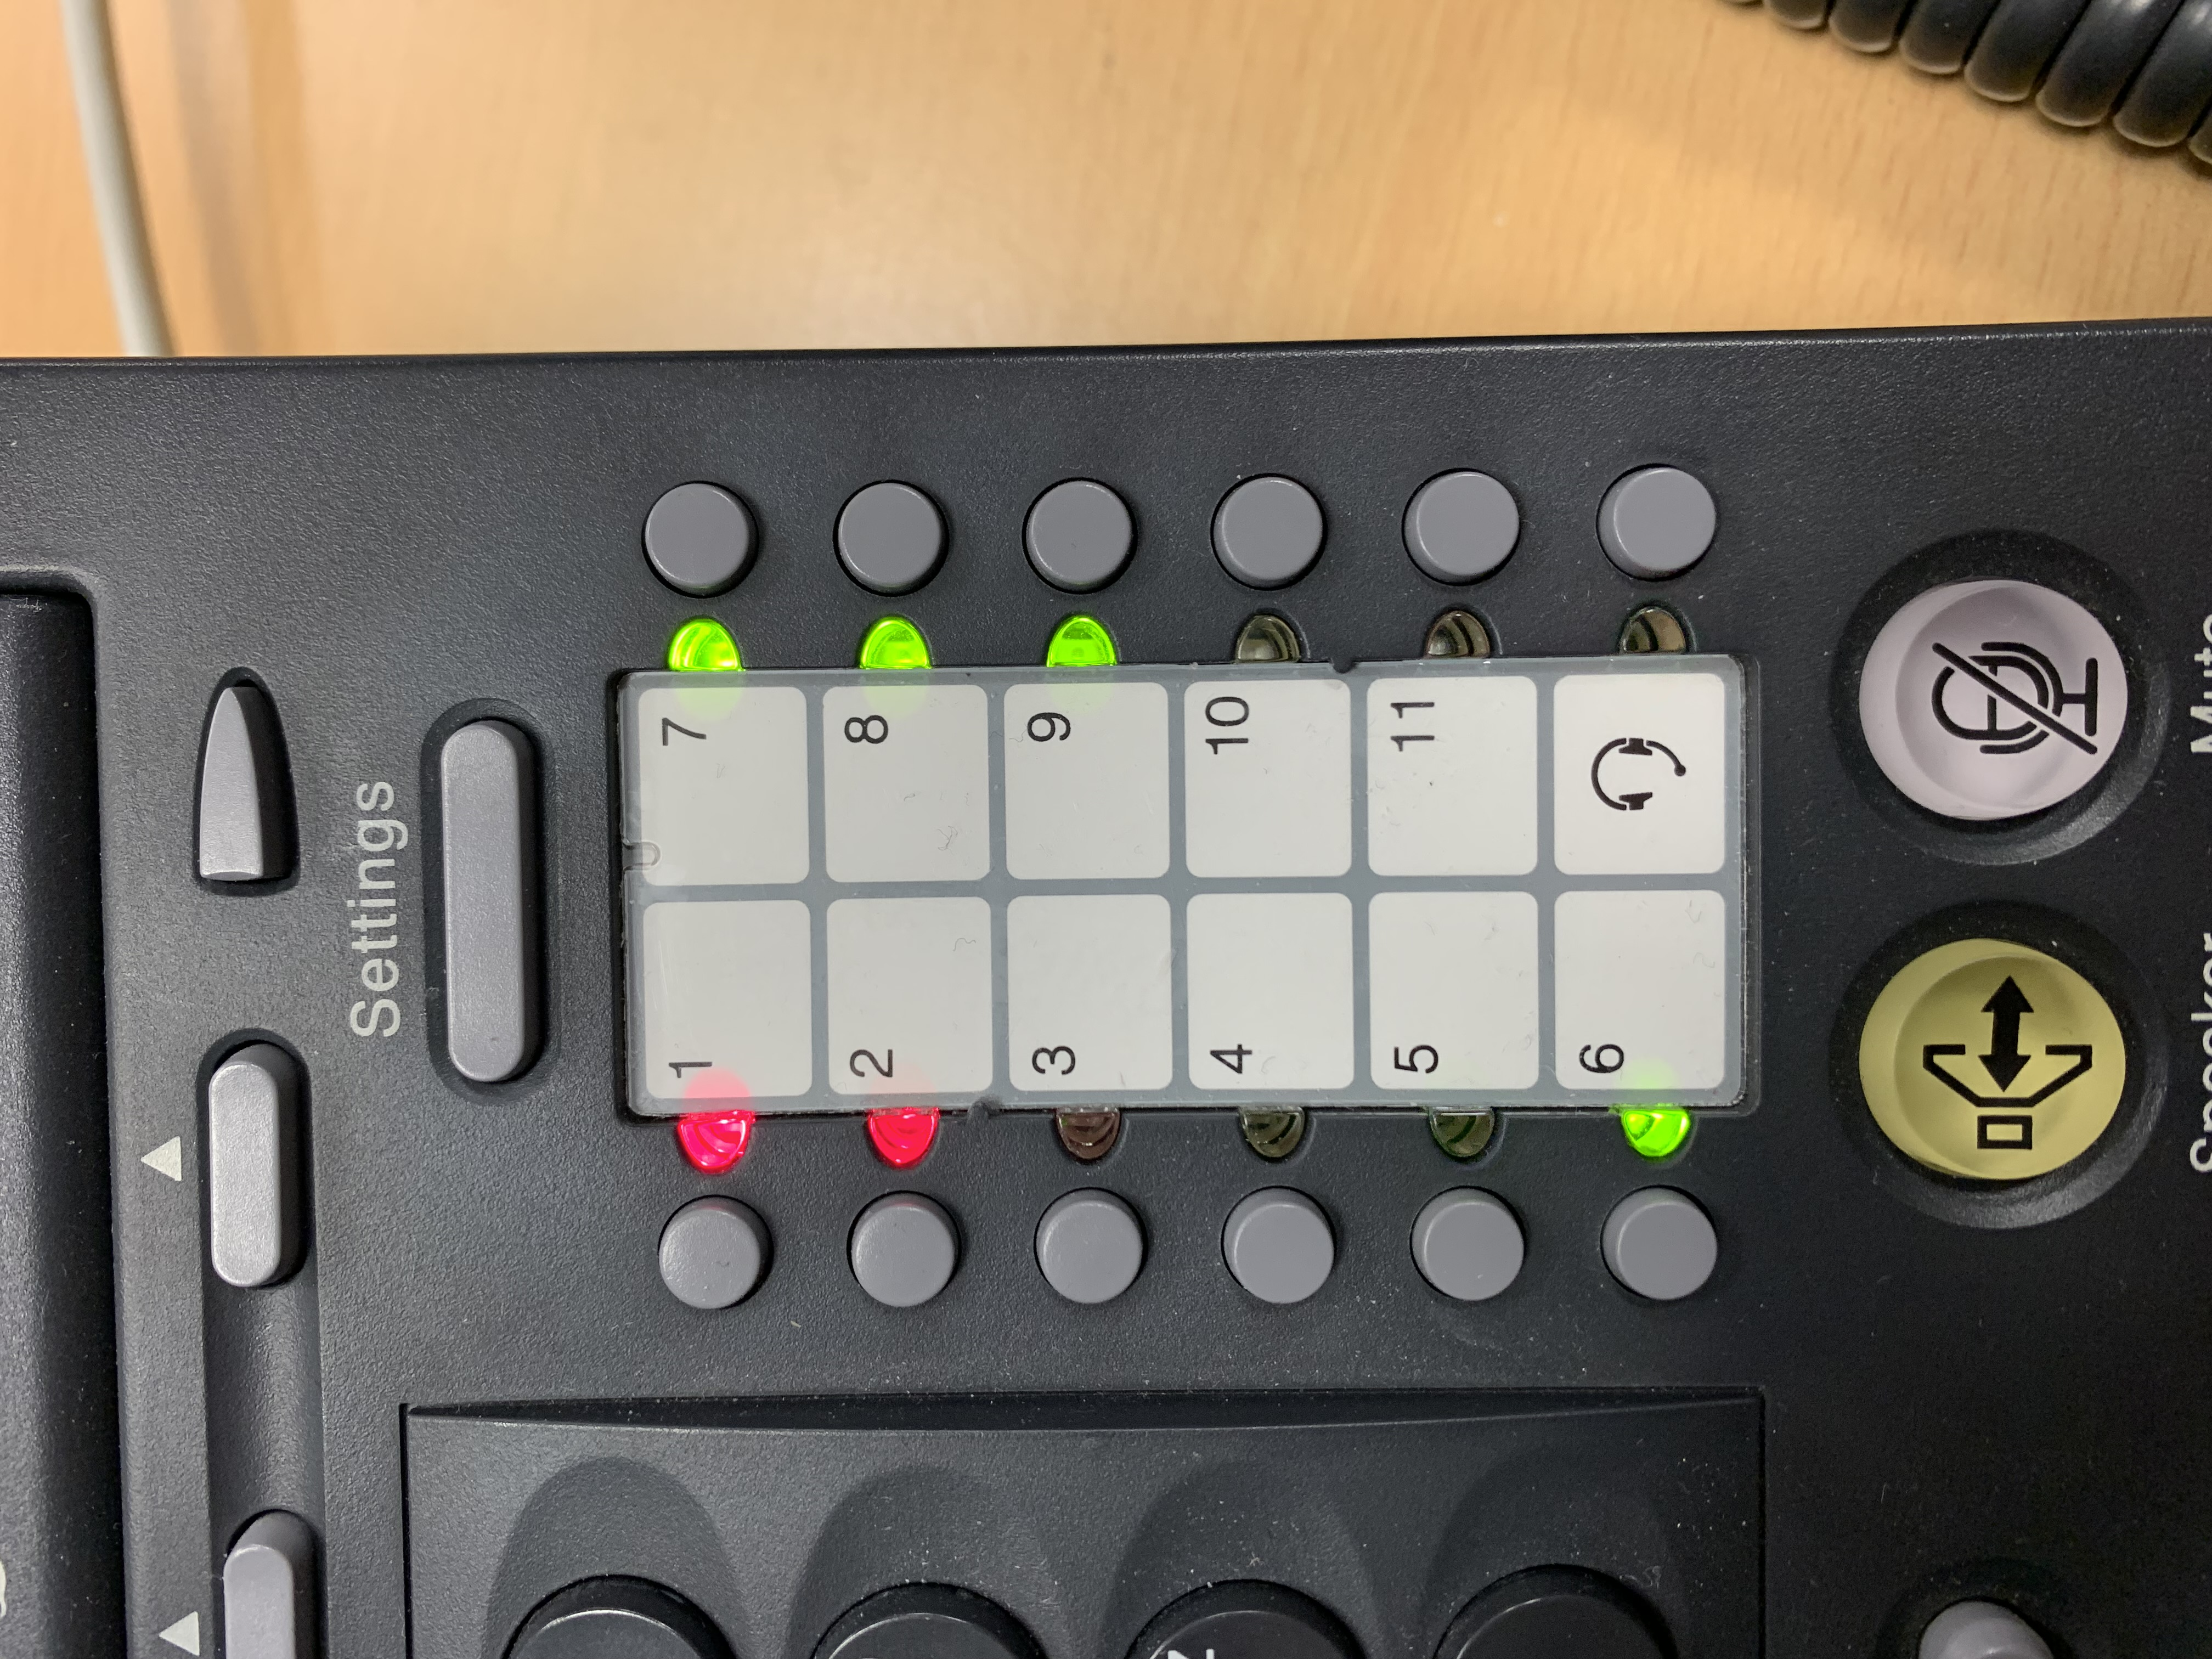
\includegraphics[width=0.7\textwidth]{img/IMG_0510.jpeg}}
		\caption{Bouton à associer}
		\label{fig:btnl}
	\end{figure}\\
	Une fois fait je choisi le numéro que je veux associer à ce bouton 
	et je valide. La procédure est exactement la même pour ajouter en raccourci
	un contact, le bouton de mise en attente ou encore la bouton pour accéder à la 
	messagerie. C'est pour cette raison que je n'expliquerai pas comment faire 
	après quand il faudra ajouter le bouton de mise en attente. 

	\subsection{Mise en attente}
	\subsubsection{Trouvez une mise en attente personnalisée}
	Pour la musique d'attente, j'ai décidé de la créer moi-même, en m'enregistrant
	avec mon téléphone. Puis que un célèbre logiciel de montage \textbf{Adobe Premiere Pro}
	j'ai rajouté une musique de fond pour donner un aspect plus professionnel.\\

	\subsubsection{Encodez la musique dans le format approprié}
	Il faut savoir que Asterisk n'accepte pas le mp3. J'ai donc converti mon fichier
	en g722. Qui est un codec que Asterisk accepte.
	Pour ce faire, je me suis rendu sur le site web \textbf{https://g711.org}.
	Sur ce dernier j'ai donc converti mon audio en g722.\\

	\subsubsection*{Définissez la musique par défaut}
	Pour définir la musique d'attente par défaut. J'ai tout simplement
	modifié premièrement dans le fichier \textbf{musiconhold.conf} le contexte 
	\textbf{[default]} :
	\begin{figure}[h]
		\centering
		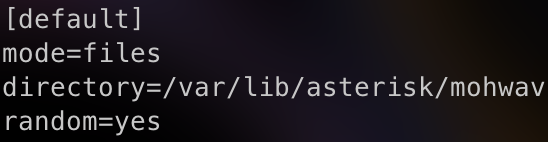
\includegraphics[width=0.7\textwidth]{img/music.png}
		\caption{Configuration du fichier musiconhold.conf}
		\label{fig:mch}
	\end{figure}\\
	Voici quelques explications pour mieux comprendre ce que ces lignes de 
	codes veulent dire :\\
	\begin{itemize}
		\item \textbf{mode=files} : définit le mode de lecture de la musique d'attente. Dans ce cas, le mode est "files", ce qui signifie que la musique sera lue à partir de fichiers audio.\\
		\item \textbf{directory=/var/lib/asterisk/mohwav} : définit le chemin du répertoire où le fichier audio de la musique d'attente est stocké. (Que j'ai au préalable crée)\\
		\item \textbf{random=yes} : définit si la musique d'attente sera jouée de manière aléatoire ou en ordre séquentiel. En utilisant "yes" pour la valeur "random", la musique d'attente sera jouée de manière aléatoire.
	\end{itemize}

	\newpage
	\subsection{Interception d'appels}
	\subsubsection{Définir un groupe d'appel Assistant et Secrétaire}
	Pour défnir un groupe d'appel comprenant l'assistante et la secrétaire, j'ai
	d'abord crée le groupe :
	\begin{figure}[h]
		\centering
		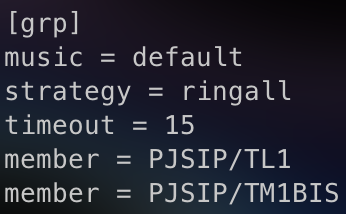
\includegraphics[width=0.6\textwidth]{img/grp.png}
		\caption{Déclaration du groupe}
		\label{fig:grph}
	\end{figure}\\
	Je viens définir une musique de prédécroché pour ce groupe. J'ai choisi 
	d'utiliser la musisque d'attente que j'ai crée précedemment pour faciliter 
	l'explication. J'ai ensuite déclaré le mode de sonnerie qui est \textbf{ringall}
	ce qui signifie que tous les membres du groupe sonneront en même temps. Puis, 
	je viens définir le temps de sonnerie et enfin, je viens définir les membres
	du groupe.\\

	\subsubsection{Activez l'interception d'appel pour le groupe précédent}
	Pour ce faire, j'ai juste rajouté ces lignes dans le contexte des déclaration
	de postes concernés dans le fichier \textbf{pjsip\_wizard.conf} :
	\begin{figure}[h]
		\centering
		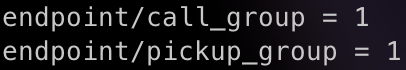
\includegraphics[width=0.6\textwidth]{img/lgrp.png}
		\caption{Activation de l'interception}
		\label{fig:lgrph}
	\end{figure}\\
	Ces lignes permettent au postes qui ont ces lignes de pouvoir intercepter les appels.

	\newpage
	\subsubsection{Validez l'interception d'appels}
	Pour pouvoir valider l'interception d'appels. J'ai généré comme vu en TP
	un appel "démo" vers mon poste TL1 à l'aide de la commande suivante : 
	\texttt{originate PJSIP/TL1 application Playback demo-congrats}. 
	Sur mon poste TM1BIS, lorsque l'appel sonne chez TL1, je peux 
	tout simplement appuyer sur \textbf{*8} pour récupérer l'appel sur TM1BIS. 

	\subsection{Enregistrement de conversation}
	\subsubsection{Activez l'enregistrement de conversation côté serveur}
	Je n'ai malheureusement pas réussi à faire fonctionner le déclenchement
	de l'enregistrement d'appel à partir du moment où on appuie sur une touche.
	Cependant, j'ai réussi à faire en sorte que les appels soient tous enregistrés
	par défauts. Pour ce faire, j'ai ajouté les lignes suivantes dans le fichier
	\textbf{extensions.conf} :
	\begin{figure}[h]
		\centering
		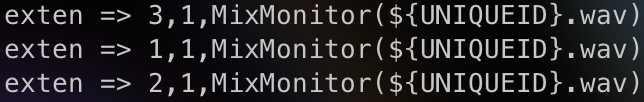
\includegraphics[width=0.7\textwidth]{img/monitor.png}
		\caption{Activation de l'enregistrement d'appels}
		\label{fig:monitor}
	\end{figure}\\
	En rajoutant ces lignes aux 3 numéros je défini donc que les appels
	passés vers les 3 numéros seront tous automatiquement enregistrés.\\

	La commande \textbf{MixMonitor(\${UNIQUEID}.wav)} :  permet d'enregistrer 
	une conversation téléphonique en cours. La commande utilise la variable 
	d'environnement \textbf{\${UNIQUEID}} pour générer un nom de fichier 
	unique pour chaque enregistrement. Le fichier enregistré aura donc un 
	nom de type \textbf{\${UNIQUEID}.wav}. La commande MixMonitor permet 
	d'enregistrer à la fois les entrées et les sorties audio de la 
	conversation téléphonique. Les fichiers d'enregistrements seront retrouvables
	dans le répertoire \textbf{/var/spool/asterisk/monitor}.\\

	\newpage
	\subsection{Prédécroché}
	\subsubsection{Enregistrez un message d'accueil personnalisé}
	Je me suis donc crée un nouveau message d'accueil différent de celui de mise
	en attente de la même manière que j'ai crée le message d'attente. Pour le message 
	de prédécroché j'ai crée une nouvelle classe dans le fichier \textbf{musiconhold.conf} :
	\begin{figure}[h]
		\centering
		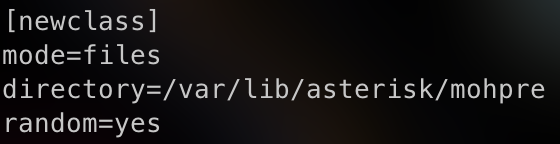
\includegraphics[width=0.7\textwidth]{img/pre.png}
		\caption{Déclaration d'un nouveau message d'accueil}
		\label{fig:new}
	\end{figure}\\
	C'est exactement le même principe que pour le message de mise en attente, 
	sauf le répertoire du fichier vu qu'il est différent est \textbf{/var/lib/asterisk/mohpre/}.
	Ensuite, dans le fichier \textbf{extensions.conf}, j'ai modifié le plan de numéroration
	pour rajouter la nouvelle classe du message d'accueil personnalisé : 
	\begin{figure}[h]
		\centering
		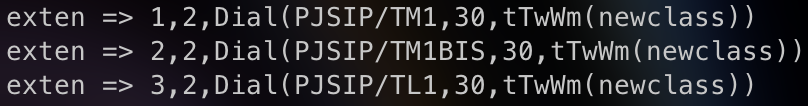
\includegraphics[width=0.8\textwidth]{img/prex.png}
		\caption{Ajout d'un nouveau message d'accueil}
		\label{fig:nexw}
	\end{figure}\\
	J'ai donc repris le plan de numérotation pour y rajouter à la fin 
	\textbf{m(newclass)} ce qui signifie tout simplement que pendant la sonnerie
	le message d'accueil associé au contexte \textbf{newclass} dans
	le fichier \textbf{musiconhold.conf} sera joué chez l'appelant.\\

\newpage
\section{Objectif 4 : Boîtes vocales}
	\subsection{Configuration serveur}
		\subsubsection{Créer une boîte vocal pour chaque utilisateurs}
		Pour créer une boite vocal à chaque utilisateur je viens définir 
		dans le contexte \textbf{[default]} du fichier \textbf{extensions.conf}
		ces lignes de code : 
		\begin{figure}[h]
			\centering
			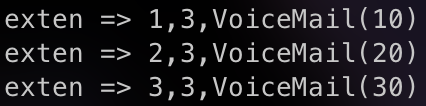
\includegraphics[width=0.8\textwidth]{img/cont.png}
			\caption{Ajout d'une boite vocal}
			\label{fig:cont}
		\end{figure}\\
		Ces lignes signifient que pour accéder par exemple à la boite vocale
		de l'utilisateur \textbf{TM1} ayant comme numéro \textbf{1}, il suffit
		de composer donc le numéro \textbf{8500} qui est le numéro de boîte vocale
		par défaut et de composer le numéro 10 qui correspond à sa boite vocale. 
		Puis, écrire le code de la boîte vocale qui est le 1-2-3-4 que je viens
		définir dans le fichier \textbf{voicemail.conf} :\\
		\begin{figure}[h]
			\centering
			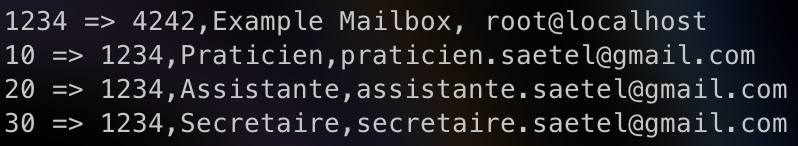
\includegraphics[width=0.8\textwidth]{img/voic.png}
			\caption{Ajout de comptes et mot de passe}
			\label{fig:voic}
		\end{figure}\\

\newpage
\section{Conclusion générale}
Ce projet fût pour nous tous une expérience très enrichissante. Nous avons
fait face à différents types de problèmes que nous avons réussi à résoudre, 
ou non. Par exemple au commencement de la SAE, nous sommes tombés face à 
notre plus gros problème qui était le téléphone Cisco. Nous avons pris énormenent
de temps à comprendre comment il était possible de les flasher. Une fois 
tout monté, à savoir le serveur TFTP. Après avoir flashé les 12 téléphones, 
nous nous sommes rendu compte qu'il n'était pas possible de les paramétrer 
pour les connecter à nos serveurs IPBX. Nous avons donc essayé dé réflechir
à des solutions, sans en trouver...\\

L'autre gros problème que j'ai eu personnellement était le message de prédécroché
en même temps que le transfert d'appels. Quand je mettais le bon paramètre pour 
avoir le transfert d'appels ça fonctionnait, et dès que je rajoutais le 
paramètre pour définir le musique de prédécroché, le transfert ne fonctionnait
plus. J'ai réussi à résoudre ce problème en modifiant juste une virgule... 
C'est-à-dire qu'initialement, j'avais dans mon plan de numérotation ceci :\\
\texttt{[...]PJSIP/TM1,30,tT,m(newclass)}. J'ai trouvé qu'en écrivant
plutôt :\\ \texttt{[...]PJSIP/TM1,30,tTm(newclass)} ça fonctionnait.
C'est une très petite et subtile différence, mais qui a su faire la différence.\\

En définitive, j'ai apprécié de projet car il était en parfaite corrélation avec
mon alternance. En tant qu'apprenti chez Orange, j'installe une offre téléphonique
qui se prénomme \textbf{Connect pro}. Cette offre est déstinée aux petites entreprises.
Elle se base sur un serveur Asterisk, et donc, tout ce que je configure chez Orange
est identique à ce que j'ai fait dans ce projet, jusqu'à même la possibilité
d'envoyer par mails les messages vocaux. La seule différence, est que chez Orange
tout a fait pour que l'installation soit la plus simple possible et rapide. 
Nous, les techniciens, passons tous par une interface graphique, tandis que 
pendant le projet tout était en ligne de commande. Je suis donc très 
content d'avoir pu voir et comprendre comment tout ce que je fais chez Orange fonctionne
réllemment en arrière plan, coté serveur. 

\end{document}